%%
%% Copyright (c) 2018-2019 Weitian LI <liweitianux@sjtu.edu.cn>
%% Creative Commons BY 4.0
%%

\chapter{再电离时期的探测}
\label{chap:detection}


\emph{\acf{eor}}是早期宇宙的一段缺乏了解的时期,目前的理论研究以及有限的观测证据表明
该时期从宇宙大爆炸之后约 \SI{300}{\Myr} 持续到约 \SI{1}{\Gyr},对应红移范围
约为 \numrange{6}{15} (参见 \citeay{koopmans2015} 及其所引文献).
充分探明并理解该时期是为进一步揭示更早的\ac{cd}和\ac{da}($z > 15$)、
建立完整的宇宙演化图景的关键环节.
在低频射电波段(约 \SIrange{50}{200}{\MHz})
探测源自再电离时期的 21\,cm 信号(即\emph{EoR 信号})
是目前研究该时期的最直接而有效的办法 \cite{madau1997,tozzi2000,furlanetto2006}.


%=====================================================================
\section{EoR 信号}
\label{sec:eor-signal}

%---------------------------------------------------------------------
\subsection{21\texorpdfstring{\,}{ }cm~谱线}
\label{sec:21cm-line}

中性氢原子的原子核(即质子)和电子均有 1/2 \ac{spin},
因此均具有相应的内禀磁矩 (intrinsic magnetic moment):
\begin{align}
  \B{\mu}_p & = |g_p| \frac{\acs{magneton-n}}{\acs{h-bar}} \B{S}_p , \\
  \B{\mu}_e & = - |g_e| \frac{\acs{magneton-b}}{\acs{h-bar}} \B{S}_e ,
\end{align}
其中
\ac{h-bar} 为\acl{h-bar},
$\ac{magneton-n} = e \,\ac{h-bar} / (2 \ac{mass-p})$ 为\acl{magneton-n},
$\ac{magneton-b} = e \,\ac{h-bar} / (2 \ac{mass-e})$ 为 \acl{magneton-b},
$g_p$ 和 $g_e$ 分别为质子和电子的 $g$ 因子,
$\B{S}_p$ 和 $\B{S}_e$ 分别为质子和电子的自旋.
电子带负电,所以磁矩方向与其自旋方向相反.
% XXX: why these symbols not printed in the list ?
\acuse{h-bar,magneton-b,magneton-n}

\begin{figure}[tbp]
  \centering
  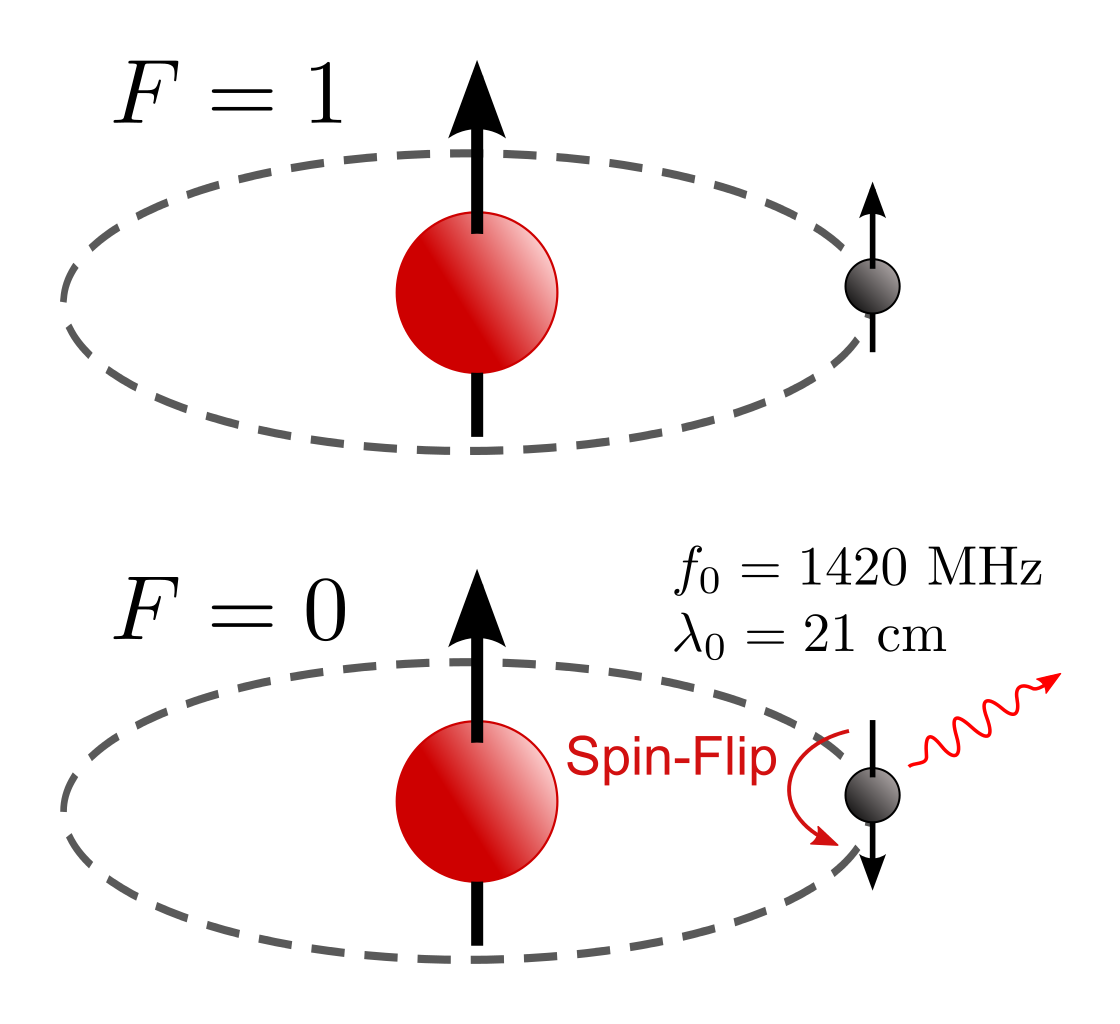
\includegraphics[width=0.5\textwidth]{hydrogen-spinflip}
  \bicaption[氢原子的自旋翻转跃迁]{%
    氢原子在基态的两个超精细分裂能级之间发生自旋翻转跃迁,产生\acs*{21cmline}.
  }{%
    An hydrogen atom makes a spin-flip transition between the two
    hyperfine levels of the ground state, emitting the \acl*{21cmline}.
    \\\textcopyright{}
    Tiltec,
    \url{https://en.wikipedia.org/wiki/File:Hydrogen-SpinFlip.svg},
    (2019-03-31), 公有领域.
  }
  \label{fig:hi-spinflip}
\end{figure}

由于质子和电子的自旋相互作用,氢原子的\ac{ground-state}
发生\ac{hyperfine-splitting}成为两个态:
(1) 质子的自旋 $\B{S}_p$ 和电子的自旋 $\B{S}_e$ 平行,总角动量 $F = 1$;
(2) $\B{S}_p$ 和 $\B{S}_e$ 反平行,总角动量 $F = 0$.
想像两个共中心的载流线圈,系统的稳定状态(即能量最低)为两个线圈的电流方向相同,
即两个载流线圈的磁矩平行.
将此应用于上述两个态,可知 $F = 1$ 态(即质子和电子的自旋反平行、磁矩平行)
的能量比 $F = 0$ 态更高 \cite{griffiths1982}.
当氢原子从 $F = 1$ 态跃迁到 $F = 0$ 态时,
将产生频率约为 $\nu = \SI{1420}{\MHz}$ 的辐射,
对应的波长约为 $\lambda = \SI{21}{\cm}$,因此称为\emph{\acf{21cmline}}.
此跃迁过程亦称为\emph{\acf{sft}},如\autoref{fig:hi-spinflip} 所示.
对于 $F = 1$ 态(即上能级),磁量子数 $m$ 可取 $\{ -1, 0, 1 \}$,
因此这个态的\ac{dod}为 3,称为\emph{\acf{triplet}};
对于 $F = 0$ 态(即下能级),磁量子数 $m$ 只能取 0,
因此这个态是\emph{\acf{singlet}}.

中性氢的 \ac{21cmline}%
首次由 H.~C. van~de~Hulst 在 1945 年提出 \cite{vanDeHulst1945},
并由 H.~I. Ewen 和 E.~M. Purcell 在 1951 年观测到 \cite{ewen1951}.
该谱线的频率是目前测量最精确的几个物理量之一 \cite{hellwig1970,essen1971}:
\begin{equation}
  \label{eq:hi-line-frequency}
  \nu_0 = \SI{1420405751.7667 +- 0.0009}{\Hz} ,
\end{equation}
对应真空中的波长为:
\begin{equation}
  \label{eq:hi-line-wavelength}
  \lambda_0 = \SI{21.1061140542}{\cm} .
\end{equation}

%---------------------------------------------------------------------
\subsection{谱线亮温度}

中性氢的 \ac{21cmline}的跃迁概率非常低,其\ac{em-spontaneous}系数 $A_{21}$ 为:
\begin{equation}
  A_{21} = \SI[separate-uncertainty=false]{2.86888(7)e-15}{\per\second} .
\end{equation}
对应的\ac{em-spontaneous}的半衰期为:
\begin{equation}
  t_{1/2} \approx 1 / A_{21}
    = \SI{3.49e14}{\second} \approx \SI{11.1}{\Myr} .
\end{equation}
该\ac{timescale}远大于典型中性氢云中的氢原子因碰撞而改变自旋的\ac{timescale},
因此中性氢的超精细结构的能级布居将由碰撞决定.

由\autoref{eq:t-excitation-def}可知,\acl{T-excitation}描述了能级的相对布居.
鉴于\ac{21cmline}源自中性氢的\ac{sft},在此情况下,
\acl{T-excitation}亦被称为\emph{\acf{T-spin}},
描述了氢原子自旋态(即\ac{singlet}和\ac{triplet})的相对布居 \cite{field1958}:
\begin{equation}
  \frac{N_2}{N_1} = \frac{g_2}{g_1}
    \exp\left( -\frac{\acs{hp} \nu_0}{\acs{kb} \acs{T-spin}} \right)
    = \frac{g_2}{g_1} \exp\left( -\frac{T_*}{\acs{T-spin}} \right),
\end{equation}
其中
$g_1 = 1$ 和 $g_2 = 3$ 分别为两个能级的\ac{dod},
$T_* \equiv \acs{hp} \nu_0 / \acs{kb} \approx \SI{68.2}{\mK}$.
在实际的天体物理应用中,均有 $\acs{T-spin} \gg T_*$,因此:
\begin{equation}
  \frac{N_2}{N_1} = \frac{g_2}{g_1} = 3 .
\end{equation}
将此代入\autoref{eq:coef-absorption-einstein3},
近似后可得中性氢云的\acl{coef-absorption}:
\begin{equation}
  \acs{coef-absorption}
    = \frac{3 \acs{hp} \acs{speed-light}^2}{32\Cpi \nu_0}
      \frac{A_{21} n_{\R{HI}}}{\acs{kb} \acs{T-spin}} \phi(\nu) ,
\end{equation}
其中 $n_{\R{HI}} = N_1 + N_2 = 4 N_1$ 为中性氢的数密度.

设一团均匀的中性氢云位于红移 $z$ 处,沿观测的视线方向的线性尺度为 $s$,
中性氢的数密度为 $n_{\R{HI}}$,
则其\acl{optical-depth} [\autoref{eq:optical-depth}] 为:
\begin{align}
  \acs{optical-depth}_{\nu_0}
    & = \int_{\R{cloud}} \acs{coef-absorption}(s') \,\D{s'}  \\
    & = \frac{3 \acs{hp} \acs{speed-light}^2}{32\Cpi \nu_0}
      \frac{A_{21}}{\acs{kb} \acs{T-spin}} \phi(\nu)
      \int_{\R{cloud}} n_{\R{HI}}(s') \,\D{s'}  \\
    & = \frac{3 \acs{hp} \acs{speed-light}^2}{32\Cpi \nu_0}
      \frac{A_{21}}{\acs{kb} \acs{T-spin}} N_{\R{HI}} \phi(\nu) ,
  \label{eq:21cm-optical-depth1}
\end{align}
其中 $N_{\R{HI}}$ 为中性氢的\ac{column-density},可进一步写成:
\begin{equation}
  \label{eq:column-density}
  N_{\R{HI}} = \acs{hi-fraction} n_{\R{HI}} s ,
\end{equation}
其中 \acs{hi-fraction} 为\acl{hi-fraction} (neutral fraction of hydrogen).

一般说来,\ac{line-profile}包含自然展宽 (natural broadening)、
热展宽 (thermal broadening)、压力展宽 (pressue broadening)、
体运动展宽 (bulk motion broadening) 等因素,
但对于 \ac{21cmline}来说,最重要的因素是宇宙膨胀引起的 Doppler 展宽.
因此,线性尺度为 $s$ 的中性氢云的速度弥散约为 $\Delta v \sim s \acs{Hz}$,
于是\ac{line-profile}可近似为:
\begin{equation}
  \phi(\nu) \sim \frac{\acs{speed-light}}{\nu \Delta v}
    \sim \frac{\acs{speed-light}}{\nu \, s \acs{Hz}} .
\end{equation}
将上式和\autoref{eq:column-density} 代入\autoref{eq:21cm-optical-depth1},
可得\acl{optical-depth}:
\begin{equation}
  \label{eq:21cm-optical-depth2}
  \acs{optical-depth}_{\nu_0}
    \approx \frac{3 \acs{hp} \acs{speed-light}^3}{32\Cpi \nu_0^2}
      \frac{A_{21}}{\acs{kb} \acs{T-spin}}
      \frac{\acs{hi-fraction} n_{\R{HI}}}{\acs{Hz}} .
\end{equation}
如果需要考虑中性氢云的\ac{v-peculiar},则其\acl{optical-depth}应为
\cite{bharadwaj2005,furlanetto2006,pritchard2012}:
\begin{equation}
  \label{eq:21cm-optical-depth3}
  \acs{optical-depth}_{\nu_0}
    \approx \frac{3 \acs{hp} \acs{speed-light}^3}{32\Cpi \nu_0^2}
      \frac{A_{21}}{\acs{kb} \acs{T-spin}}
      \frac{\acs{hi-fraction} n_{\R{HI}}}{
        (1+z) (\partial v_{\parallel} / \partial r_{\parallel})} ,
\end{equation}
其中 $(\partial v_{\parallel} / \partial r_{\parallel})$ 是\ac{v-proper}
沿视线方向的梯度.
此外,通常均有\acl{optical-depth} $\acs{optical-depth}_{\nu0} \ll 1$
\cite{madau1997,furlanetto2006,pritchard2010mn}.

\begin{figure}[tbp]
  \centering
  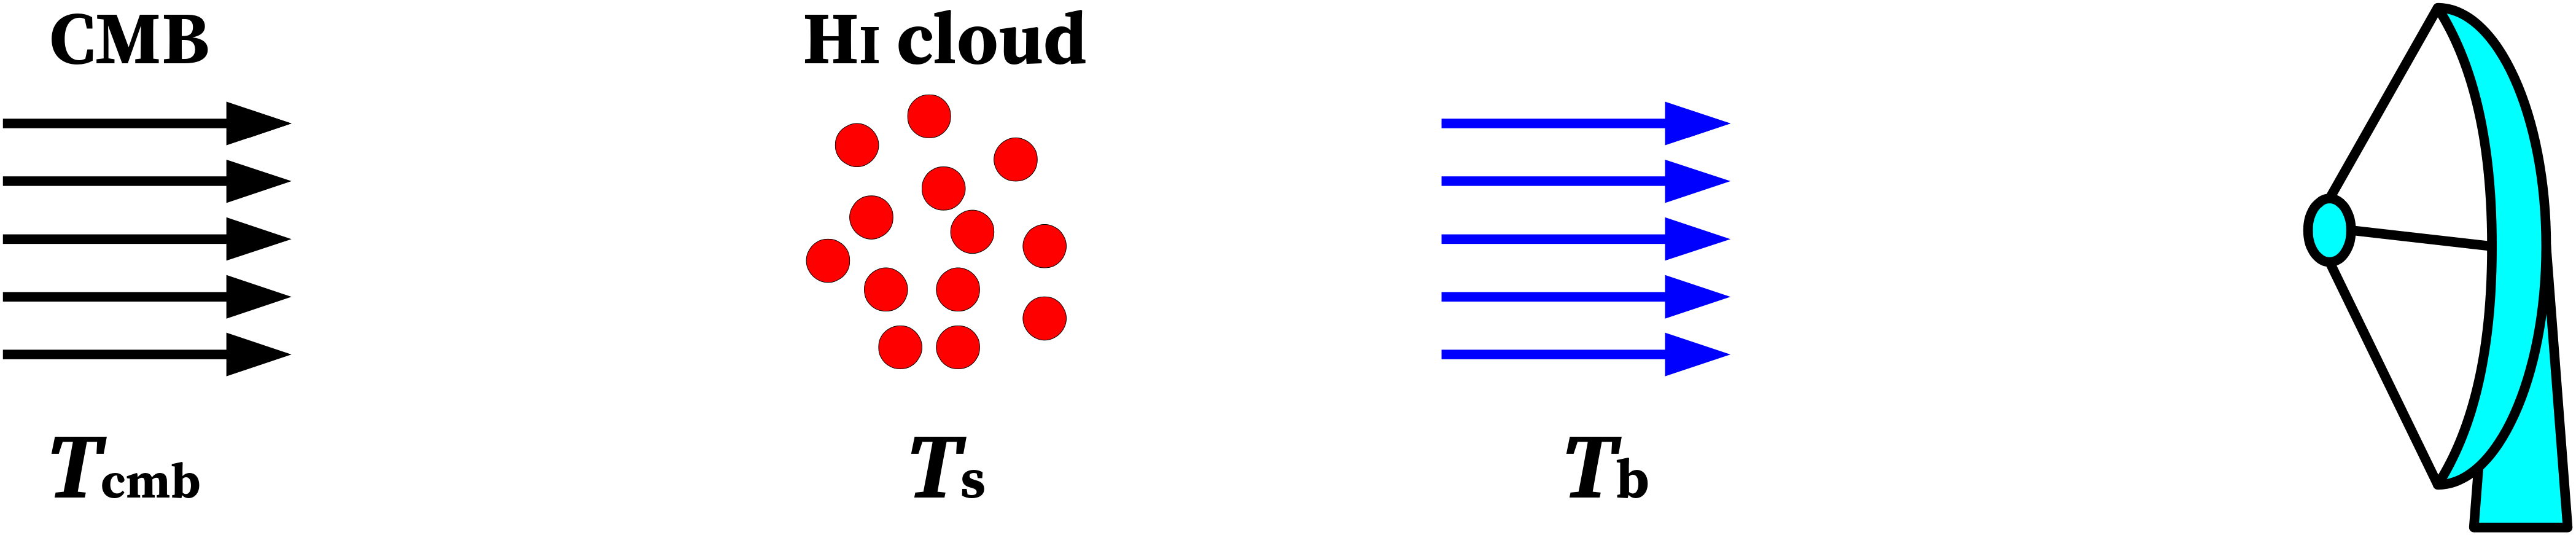
\includegraphics[width=0.9\textwidth]{21cm-radiative-transfer}
  \bicaption[CMB 辐射穿过中性氢云的辐射转移示意图]{%
    CMB 辐射穿过中性氢云的辐射转移示意图:
    从\acl*{T-spin}为 \acs*{T-spin} 的中性氢云出射的
    CMB 辐射的温度为 \acs*{T-b}.
  }{%
    An illustration of the radiative transfer process:
    the CMB radiation goes through a cloud of hydrogen with
    spin temperature \acs*{T-spin} and emerges with a temperature
    \acs*{T-b} measured by a telescope.
    \\\textcopyright{}
    \citeay{zaroubi2013}, \S\,4.1.
    [经过了左右翻转]
  }
  \label{fig:21cm-cmb-rt}
\end{figure}

在实际观测中,需要考虑 \ac{cmb} 辐射穿过中性氢云的转移过程,
如\autoref{fig:21cm-cmb-rt} 所示.
考虑一团处于热平衡状态、\acl{T-spin}为 \acs{T-spin}、位于红移 $z$ 处的中性氢云,
结合 Kirchhoff 定律 [\autoref{eq:kirchhoff-law}] 可得\ac{rt}方程为:
\begin{equation}
  \diff{\acs{I-nu}}{s}
    = -\acs{coef-absorption}\,\acs{I-nu} + \acs{coef-emission}
    = -\acs{coef-absorption}\,[\acs{I-nu} - B_{\nu}(\acs{T-spin})] ,
\end{equation}
其中
$B_{\nu}(\acs{T-spin})$ 是温度为 \acs{T-spin} 的黑体辐射谱 [\autoref{eq:planck}].
利用 Rayleigh--Jeans 近似 [\autoref{eq:rj-approx}]
将 \acs{I-nu} 表示为\acl{T-b} $\acs{T-b}(\nu)$:
\begin{equation}
  \diff{\acs{T-b}}{s}
    = -\acs{coef-absorption} [\acs{T-b} - \acs{T-spin}] .
\end{equation}
根据\acl{optical-depth}的定义 [\autoref{eq:optical-depth}]
有 $\D{\tau'} = -\acs{coef-absorption}\,\D{s}$,
代入上式可得:
\begin{equation}
  \diff{\acs{T-b}}{\tau'} = \acs{T-b} - \acs{T-spin} .
\end{equation}
上式两边均乘上 $\Ce^{-\tau'}\,\D{\tau'}$ 并积分:
\begin{equation}
  \acs{T-b}\,\Ce^{-\tau'}\,\Big|_0^{\tau_{\nu_0}}
      - \int_0^{\tau_{\nu_0}} \acs{T-b}\,\D{(\Ce^{-\tau'})}
    = \int_0^{\tau_{\nu_0}} \acs{T-b}\,\Ce^{-\tau'}\,\D{\tau'}
      + \acs{T-spin} \int_0^{\tau_{\nu_0}} \Ce^{-\tau'}\,\D{\tau'} ,
\end{equation}
可得:
\begin{equation}
  \acs{T-b}(\tau'=\tau_{\nu_0})\,\Ce^{-\tau_{\nu}} - \acs{T-b}(\tau'=0)
    = \acs{T-spin} (\Ce^{-\tau_{\nu}} - 1) ,
\end{equation}
其中 $\acs{T-b}(\tau'=\tau_{\nu_0}) = T_{\R{cmb}}(z)$
为辐射入射中性氢云时的亮温度,
于是获得从中性氢云出射 ($\tau = 0$) 的辐射亮温度 $\acs{T-b}(\nu_0)$ 为:
\begin{equation}
  \acs{T-b}(\nu_0)
    = \acs{T-spin} (1 - \Ce^{-\tau_{\nu_0}})
      + T_{\R{cmb}}(z) \,\Ce^{-\tau_{\nu_0}} .
\end{equation}
其中 $T_{\R{cmb}}(z)$ 为 \ac{cmb} 辐射在红移 $z$ 时的\ac{comoving-frame}
中的亮温度:
\begin{align}
  T_{\R{cmb}}(z)
    & = T_{\R{cmb}}(z=0)\,(1+z)  \\
    & = 2.73 (1+z) \quad [\si{\kelvin}] ,
\end{align}
类似地,宇宙膨胀的红移效应将中性氢的 \ac{21cmline}红移至频率 $\nu = \nu_0/(1+z)$,
同时观测到的中性氢云的亮温度将为:
\begin{equation}
  T_b^{\R{obs}}(\nu) = \frac{T_b(\nu_0)}{1 + z} .
\end{equation}
目前观测 \ac{21cmline}的策略是测量其相对于 \ac{cmb} 背景辐射的差异,
即\emph{\acf{dT-b}}.
综上,并结合\autoref{eq:21cm-optical-depth3},最终可得待探测的 \emph{EoR 信号}为:
\begin{align}
  \acs{dT-b}(\nu)
    & = \frac{T_b(\nu_0)}{1 + z} - T_{\R{cmb}}(z=0)  \\
    & = \frac{\acs{T-spin} - T_{\R{cmb}}(z)}{1+z}
      (1 - \Ce^{-\acs{optical-depth}_{\nu_0}})  \\
    & \approx \frac{\acs{T-spin} - T_{\R{cmb}}(z)}{1+z}
      \acs{optical-depth}_{\nu_0}  \\
    & \approx \frac{3 \acs{hp} \acs{speed-light}^3 A_{21}}{
      32\Cpi \nu_0^2 \,\acs{kb}}
      \frac{\acs{hi-fraction} n_{\R{HI}}}{
        (1+z)^2 (\partial v_{\parallel} / \partial r_{\parallel})}
      \left[ 1 - \frac{T_{\R{cmb}}(z)}{\acs{T-spin}} \right] .
    \label{eq:eor-signal1}
\end{align}

由于再电离时期的红移较大 ($z \gtrsim 6$),
因此 Hubble 常数 [\autoref{eq:hubble-z}] 可近似为:
\begin{equation}
  \acs{Hz} = \acs{H0} \sqrt{\acs{Om0} (1+z)^3 + \acs{Ol0}}
    \approx \acs{H0} \Omega_m^{1/2} (1+z)^{3/2} .
\end{equation}
结合\autoref{eq:omega-m-z},可得红移为 $z$ 时的宇宙重子物质密度参数为:
\begin{equation}
  \acs{Ob0}(z) = \frac{\acs{Ob0}}{\acs{Om0}} \acs{Om0}(z)
    \approx \frac{\acs{Ob0}}{\acs{Om0}} .
\end{equation}
再利用当地的重子物质\ac{overdensity},即
\begin{equation}
  1 + \delta_b = \frac{\rho_b}{\overline{\rho}_b}
    \approx \frac{n_{\R{HI}} \acs{mass-p}}{\acs{Ob0}(z) \acs{rho-crit}(z)} ,
\end{equation}
其中 $\acs{rho-crit}(z)$ 为\acl{rho-crit} [\autoref{eq:rho-crit}],
可将中性氢的数密度 $n_{\R{HI}}$ 表示为:
\begin{align}
  n_{\R{HI}}
    & \approx \frac{1+\delta_b}{\acs{mass-p}} \frac{\acs{Ob0}}{\acs{Om0}}
      \frac{3 H^2(z)}{8 \Cpi \acs{G}}  \\
    & \approx \frac{3 \acs{H0}}{8\Cpi\acs{mass-p}\acs{G}}
      \frac{\acs{Ob0}}{\Omega_m^{1/2}} (1+\delta_b) (1+z)^{3/2} \acs{Hz} .
\end{align}
将上式代入\autoref{eq:eor-signal1},可得 EoR 信号的最终表达式:
\begin{align}
  \acs{dT-b}(\nu)
    & \approx \frac{9 \acs{hp} \acs{speed-light}^3 A_{21}}{
      256\Cpi^2 \nu_0^2 \,\acs{kb} \acs{mass-p} \acs{G}}
      \frac{\acs{H0} \acs{Ob0}}{\Omega_m^{1/2}}
      \acs{hi-fraction} (1+\delta_b) (1+z)^{1/2}
      \left[ 1 - \frac{T_{\R{cmb}}(z)}{\acs{T-spin}} \right]
      \left[ \frac{\acs{Hz} / (1+z)}{
        \partial v_{\parallel} / \partial r_{\parallel}} \right]
  \label{eq:eor-signal2}  \\
    & \approx \left( \SI{38}{\mK} \right)
      \acs{hi-fraction} (1+\delta_b)
      \left( \frac{1+z}{10} \right)^{1/2}
      \left( \frac{0.27}{\acs{Om0}} \right)^{1/2}
      \left( \frac{\acs{Ob0} \acs{h}^2}{0.023} \right)
      \left[ 1 - \frac{T_{\R{cmb}}(z)}{\acs{T-spin}} \right]
      \left[ \frac{\acs{Hz} / (1+z)}{
        \partial v_{\parallel} / \partial r_{\parallel}} \right] .
  \label{eq:eor-signal3}
\end{align}

%---------------------------------------------------------------------
\subsection{亮温度的演化}

由\autoref{eq:eor-signal2} 易知,\acl{T-spin} \acs{T-spin}
对 EoR 信号 $\acs{dT-b}(\nu)$ 的强度起关键作用.
当 $\acs{T-spin} > T_{\R{cmb}}(z)$ 时,$\acs{dT-b}(\nu) > 0$ 为发射信号,
并且当 $\acs{T-spin} \gg T_{\R{cmb}}(z)$ 时 $\acs{dT-b}(\nu)$ 达到饱和;
当 $\acs{T-spin} < T_{\R{cmb}}(z)$ 时,$\acs{dT-b}(\nu) < 0$ 表现为吸收信号.
\acl{T-spin} \acs{T-spin} 主要由以下三个过程决定:
\begin{itemize}
  \item CMB 辐射光子被中性氢吸收或者使中性氢产生\ac{em-stimulated},
    该过程使得 \acs{T-spin} 与 $T_{\R{cmb}}(z)$ 相互耦合;
  \item 中性氢原子与其他原子或电子碰撞,
    这个过程将 \acs{T-spin} 耦合到介质的\acl{T-kinetic} \acs{T-kinetic};
  \item 中性氢原子与 Lyα 光子发生\ac{resonant-scattering}而改变自旋状态,
    即 Wouthuysen--Field 效应 \cite{wouthuysen1952,field1958},
    该过程将 \acs{T-spin} 与 Lyα 辐射的\ac{T-color}关联起来.
\end{itemize}

\begin{figure}[tbp]
  \centering
  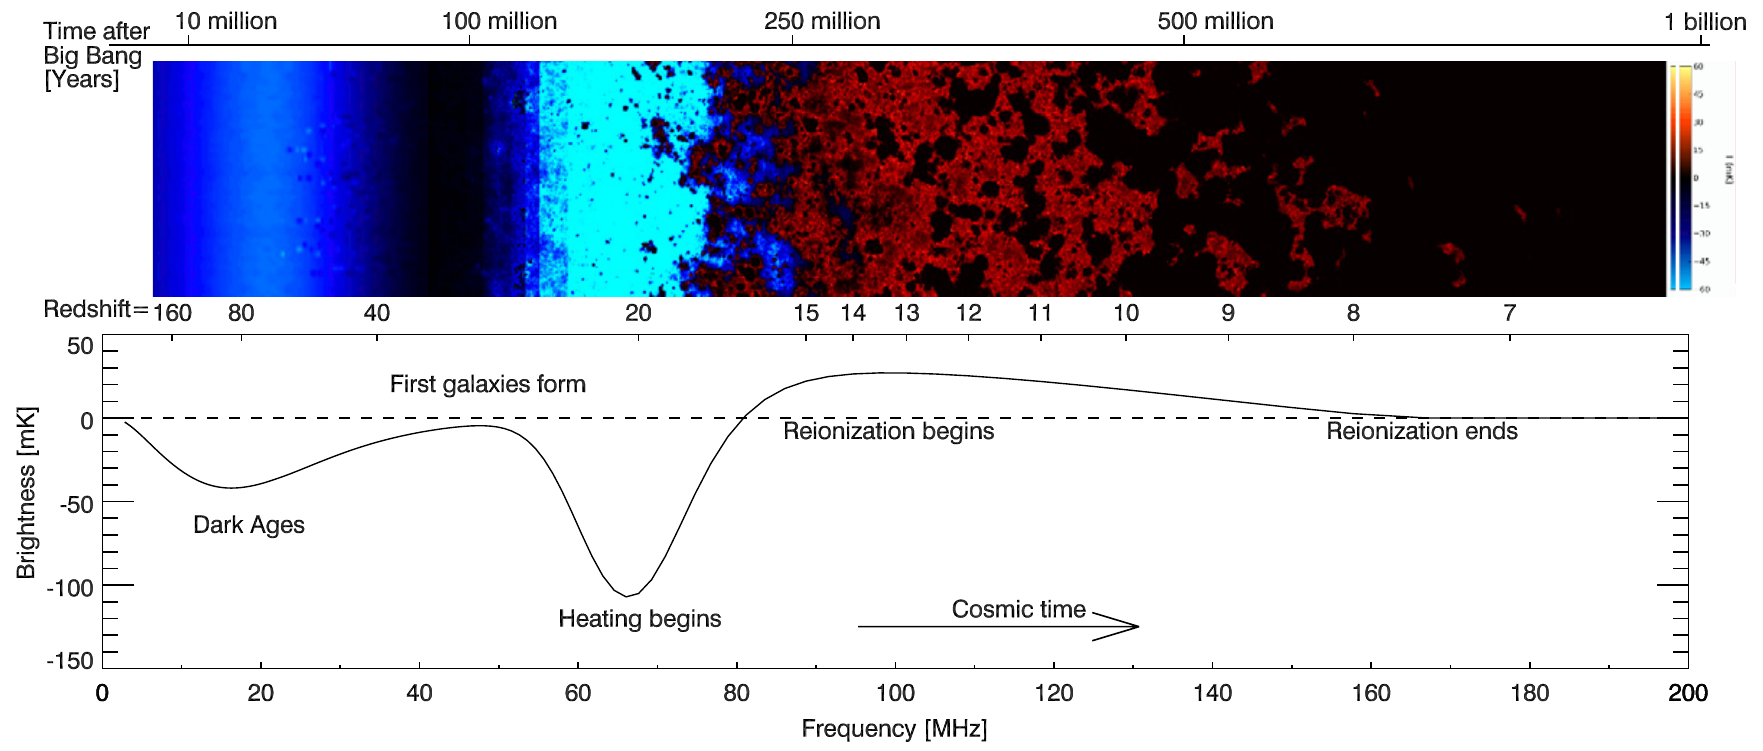
\includegraphics[width=\textwidth]{eor-signal-evolution}
  \bicaption[EoR 信号的平均强度的演化示意图]{%
    \uline{(上栏)}
    宇宙学模拟\cite{santos2008}给出的 EoR 信号的演化过程.
    \uline{(下栏)}
    理论模型给出的 EoR 信号的全天平均强度
    $\delta\overline{T}_b$ 的变化过程.
  }{%
    \emph{(Upper)} The time evolution of the EoR signal dervied from
    a cosmological simulation \cite{santos2008}.
    \emph{(Lower)} The expected evolution of the sky-averaged EoR signal
    $\delta\overline{T}_b$.
    \\\textcopyright{}
    \citeay{pritchard2012}, \S\,1.
  }
  \label{fig:eor-signal-evo}
\end{figure}

上述过程与宇宙的再电离过程、第一代天体的形成、星系的形成与演化等环节密切相关,
因此 EoR 信号随宇宙的演化而发生复杂的变化,并反映在其频谱上
(不同的频率对应于不同的红移,即宇宙年龄),如\autoref{fig:eor-signal-evo} 所示.
EoR 信号的完整演化过程可大致分为以下几个阶段 \cite{pritchard2012}:
\begin{enumerate}
  \item $200 \lesssim z \lesssim 1100$:
    \ac{recomb}之后残留的自由电子通过 Compton 散射使气体与 \ac{cmb} 保持热耦合,
    即有 $\acs{T-kinetic} = T_{\R{cmb}}$.
    因气体密度高,有效的碰撞使得 $\acs{T-spin} = T_{\R{cmb}}$,
    所以此阶段没有可探测的 EoR 信号 ($\delta\overline{T}_b = 0$).

  \item $40 \lesssim z \lesssim 200$:
    气体绝热冷却 $\acs{T-kinetic} \propto (1+z)^2$
    从而有 $\acs{T-kinetic} < T_{\R{cmb}}$,但气体中的碰撞仍然足够有效,
    因此 $\acs{T-spin} = \acs{T-kinetic} < T_{\R{cmb}}$,
    所以 EoR 信号在此阶段为吸收信号 ($\delta\overline{T}_b < 0$).

  \item $z_* \lesssim z \lesssim 40$:
    ($z_*$ 对应第一代天体形成的时刻.)
    气体密度随着宇宙膨胀而显著降低,导致碰撞耦合不如 \ac{cmb} 辐射的耦合有效,
    因此有 $\acs{T-spin} = T_{\R{cmb}}$,所以此阶段无可探测的 EoR 信号.

  \item $z_{\alpha} \lesssim z \lesssim z_*$:
    ($z_{\alpha}$ 对应 Lyα 光子的耦合达到饱和的时刻.)
    第一代天体开始形成,辐射 Lyα 光子和 X 射线,
    并将 \acs{T-spin} 与冷气体的温度耦合在一起,
    即 $\acs{T-spin} \sim \acs{T-kinetic} < T_{\R{cmb}}$,
    因此该阶段可探测到 EoR 吸收信号 ($\delta\overline{T}_b < 0$).

  \item $z_h \lesssim z \lesssim z_{\alpha}$:
    ($z_h$ 对应气体被加热至与 $T_{\R{cmb}}$ 相同温度的时刻.)
    随着星系和宇宙大尺度结构的形成,气体逐渐被加热,
    对 \acs{T-spin} 的影响也越来越显著.
    在气体温度 $\acs{T-kinetic} \sim \acs{T-spin} < T_{\R{cmb}}$
    的这一阶段,可继续探测到 EoR 吸收信号 ($\delta\overline{T}_b < 0$).

  \item $z_t \lesssim z \lesssim z_h$:
    随着气体被继续加热,$\acs{T-kinetic} \sim \acs{T-spin} > T_{\R{cmb}}$,
    因此 EoR 信号从上一阶段的吸收信号转变为发射信号 ($\delta\overline{T}_b > 0$).
    直到 $z_t$ 时刻,气体的温度已足够高
    $\acs{T-kinetic} \sim \acs{T-spin} \gg T_{\R{cmb}}$,
    EoR 信号的强度达到饱和.

  \item $z_r \lesssim z \lesssim z_t$:
    在此阶段,气体的温度 ($\acs{T-kinetic} \sim \acs{T-spin} \gg T_{\R{cmb}}$)
    对 EoR 信号的影响已变得不重要,
    因此 EoR 信号的强度将主要取决于\acl{hi-fraction} \acs{hi-fraction}.
    随着再电离的进行,\acs{hi-fraction} 逐渐变小,EoR 信号的强度也随之减小,
    直到 $z_r$ 时再电离结束.

  \item $z \lesssim z_r$:
    再电离结束后,残留的 21\,cm 信号主要源自一些塌缩的中性氢岛,比如\ac{dla}.
\end{enumerate}

由于缺乏足够的观测证据的约束,上述阶段的划分仍有很大的不确定性,
相邻阶段之间可能有显著交叠,甚至 $z_{\alpha}$ 和 $z_h$ 的次序可能需要修正
\cite{nusser2005,pritchard2012}.
基于目前非常有限的观测证据,理论模型显示宇宙的再电离过程约从红移 $z \sim 15$ 开始,
应在红移 $z > 6.5$ 之前完成,但也不能显著早于 $z \sim \numrange{7}{8}$
\cite{choudhury2006,pritchard2010mn}.

%=====================================================================
\section{功率谱}
\label{sec:ps}

由于宇宙膨胀,位于红移 $z$ 处的中性氢云产生的 \ac{21cmline}将被红移至频率
$\nu = \nu_0 / (1 + z)$,其中 $\nu_0$ 为 \ac{21cmline}的本征频率
[\autoref{eq:hi-line-frequency}].
据此,对于某一视线方向,通过在不同的频率测量 \ac{21cmline},
便可以相应地重建出中性氢在该视线上的分布情况.
对于一个天区,如果获得 \ac{21cmline}在一段频率内的图像 $I(\B{\theta},\nu)$,
即\ac{imgcube},便可以重建出中性氢的三维分布,
其中两个空间维度 $\B{\theta}$ 映射到中性氢的横向距离,
频率维度 $\nu$ 对应中性氢的视向距离.
此即\emph{\acf{21cm-tomography}} \cite{mellema2015}.

对 EoR 信号的\ac{imgcube} $I(\B{\theta},\nu)$ 进行三维 Fourier 变换:
\begin{equation}
  \label{eq:ft3d}
  \tilde{I}(\B{u}, \eta) =
    \int I(\B{\theta},\nu) \exp[ -2\Cpi\Ci (\B{u}\cdot\B{\theta} + \eta\nu) ]
    \,\mathrm{d}^2\B{\theta}\,\D{\nu} ,
\end{equation}
其中 $(\B{u}, \eta) = 1 / (\B{\theta}, \nu)$ 分别是
空间维度 $\B{\theta}$ 和频率维度 $\nu$ 的 Fourier 对偶 (dual).
于是可得由下式定义的三维\ac{ps} $\bar{P}(\B{u}, \eta)$:
\begin{equation}
  \label{eq:ps3d}
  \langle \tilde{I}(\B{u}, \eta) \, \tilde{I}^*(\B{u}', \eta') \rangle
    \equiv \bar{P}(\B{u}, \eta) \delta(\B{u}-\B{u}') \delta(\eta-\eta') ,
\end{equation}
其中 $\tilde{I}^*$ 为 $\tilde{I}$ 的\ac{cconj}.

然而,宇宙学研究中通常使用\ac{comoving-frame}以及一种不同的 Fourier 约定.
一个三维场 $T(\B{r}_{\bot}, r_{\parallel})$ 的 Fourier 变换为:
\begin{equation}
  \label{eq:ft3d-k}
  \tilde{T}(\B{k}_{\bot}, k_{\parallel}) =
    \int T(\B{r}_{\bot}, r_{\parallel})
    \exp[ -\Ci (\B{k}_{\bot} \cdot \B{r}_{\bot}
      + k_{\parallel} r_{\parallel}) ]
    \,\mathrm{d}^2\B{r}_{\bot} \,\D{r}_{\parallel} ,
\end{equation}
其中 $(\B{r}_{\bot}, r_{\parallel})$ 分别表示
垂直于视线方向和平行于视线方向的\acl{distance-comoving},
$(\B{k}_{\bot}, k_{\parallel}) = 2\Cpi / (\B{r}_{\bot}, r_{\parallel})$
分别表示 Fourier 空间中垂直于视线方向和平行于视线方向的\ac{wavenumber}.
注意,对比\autoref{eq:ft3d},上式的相位因子少了系数 $2\Cpi$.
于是,相应的逆 Fourier 变换为:
\begin{equation}
  T(\B{r}_{\bot}, r_{\parallel}) =
    \frac{1}{(2\Cpi)^3} \int \tilde{T}(\B{k}_{\bot}, k_{\parallel})
    \exp[ \Ci (\B{k}_{\bot} \cdot \B{r}_{\bot}
      + k_{\parallel} r_{\parallel}) ]
    \,\mathrm{d}^2\B{k}_{\bot} \,\D{k}_{\parallel} ,
\end{equation}
三维功率谱 $P(\B{k}_{\bot}, k_{\parallel})$ 则由下式给出:
\begin{equation}
  \label{eq:ps3d-k}
  \langle \tilde{T}(\B{k}_{\bot}, k_{\parallel})
      \, \tilde{T}^*(\B{k}'_{\bot}, k'_{\parallel}) \rangle
    \equiv (2\Cpi)^3 P(\B{k}_{\bot}, k_{\parallel})
      \delta(\B{k}_{\bot} - \B{k}'_{\bot})
      \delta(k_{\parallel} - k'_{\parallel}) .
\end{equation}

利用 \ac{21cmline}的观测频率、红移、\acl{distance-comoving}之间的对应关系,可得:
\begin{align}
  \B{r}_{\bot} & = \acs{distance-comoving}(z) \,\B{\theta} , \\
  \Delta r_{\parallel}
    & = \frac{\acs{speed-light}}{\nu_0 \acs{H0}}
      \frac{(1+z)^2}{\acs{Ez}} \Delta \nu ,
\end{align}
其中 $\acs{distance-comoving}(z)$ 为\acl{distance-comoving}
[\autoref{eq:distance-comoving}],
\acs{Ez} 为\acl{Ez} [\autoref{eq:Ez}].
可选取合适的坐标系原点,使得上式经过
$(\Delta r_{\parallel}, \Delta\nu) \to (r_{\parallel}, \nu)$
替换后仍然成立.
对比\autoref{eq:ft3d} 和\autoref{eq:ft3d-k},可得:
\begin{align}
  \B{k}_{\bot} & = \frac{2\Cpi}{\acs{distance-comoving}(z)} \B{u} , \\
  k_{\parallel} & =
    \frac{2\Cpi \nu_0 \acs{H0}\acs{Ez}}{\acs{speed-light} (1+z)^2} \eta ,
\end{align}
据此,可知\autoref{eq:ps3d} 和\autoref{eq:ps3d-k} 给出的三维功率谱
之间的转换关系为:
\begin{equation}
  P(\B{k}_{\bot}, k_{\parallel}) =
    \frac{\acs{speed-light} (1+z)^2 D_{\!C}^2(z)}{\nu_0 \acs{H0}\acs{Ez}}
    \bar{P}(\B{u}, \eta) .
\end{equation}
更多细节可参考 \citeay{liu2014} 的附录 A.
由\autoref{eq:ps3d-k} 给出的 EoR 信号的三维功率谱
$P(\B{k}_{\bot}, k_{\parallel})$ 的常用单位是 [\si{\mK\squared\Mpc\cubed}],
实际研究中更常用到的是相对应的去量纲形式 \cite{peacock1996}:
\begin{equation}
  \label{eq:ps3d-k2}
  \Delta^2(\B{k}_{\bot}, k_{\parallel})
    \equiv \frac{k^3}{2\Cpi^2} P(\B{k}_{\bot}, k_{\parallel}) ,
\end{equation}
此形式的功率谱 $\Delta^2(\B{k}_{\bot}, k_{\parallel})$
的单位变成 [\si{\mK\squared}].

\begin{figure}[tbp]
  \centering
  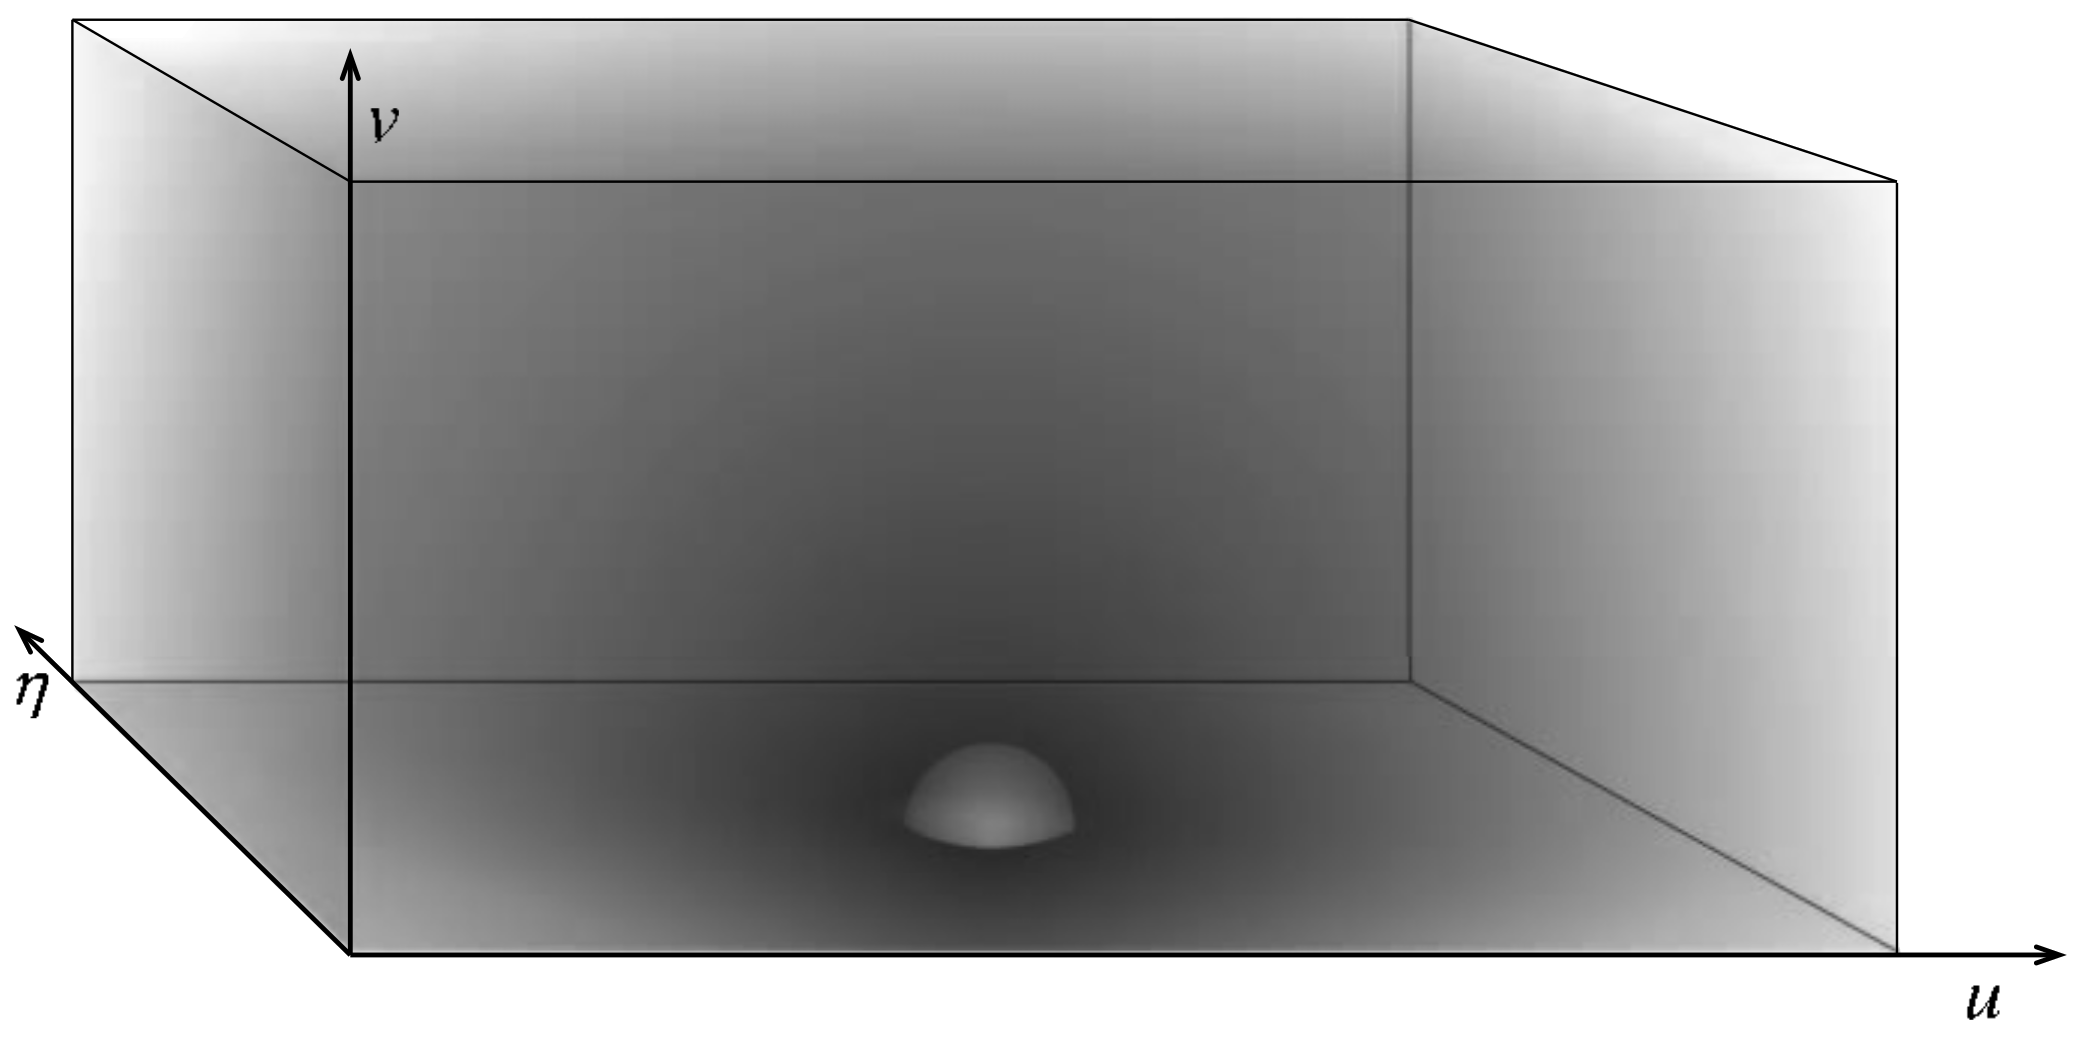
\includegraphics[width=0.5\textwidth]{EoR-fourier}%
  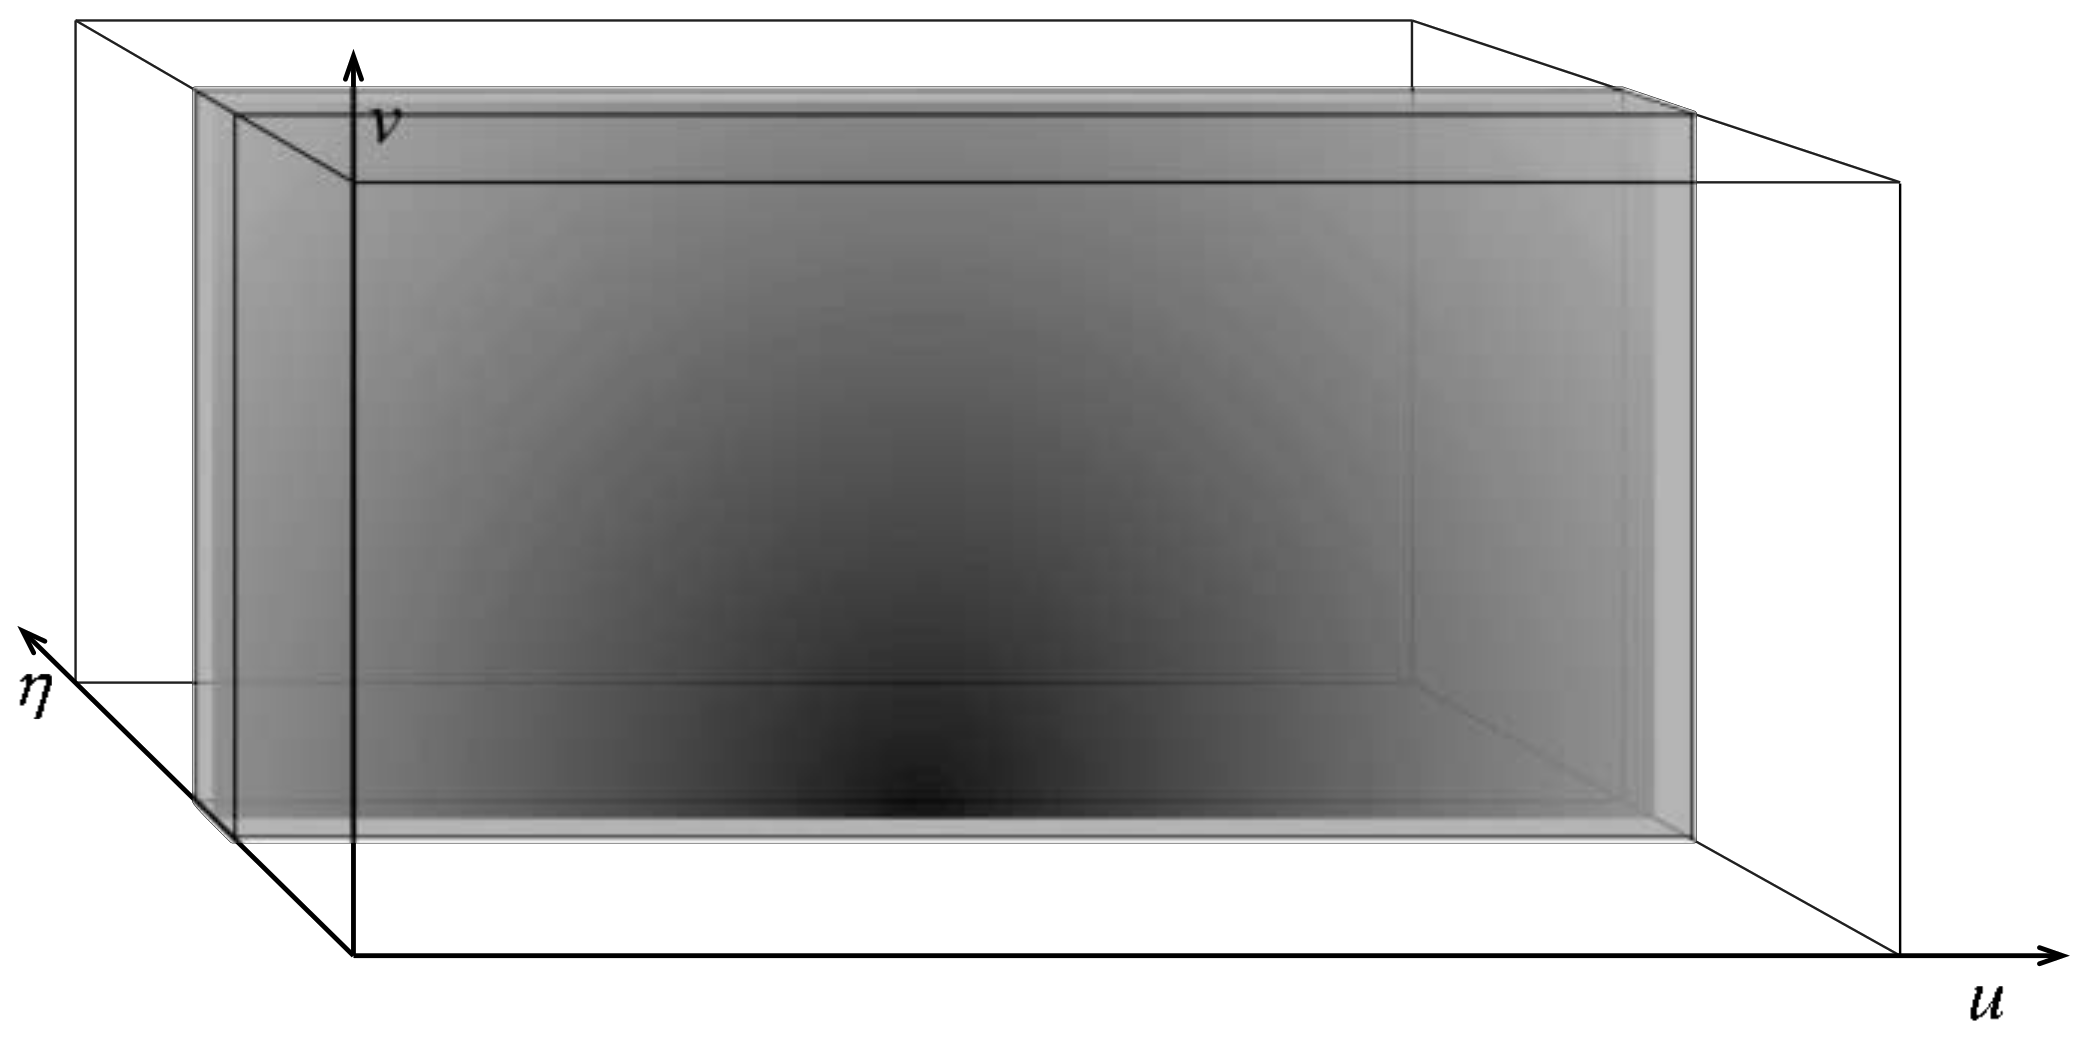
\includegraphics[width=0.5\textwidth]{foreground-fourier}
  \bicaption[EoR 信号和前景的三维功率谱示意图]{%
    \uline{(左栏)} EoR 信号的三维功率谱示意图,呈球对称分布.
    \uline{(右栏)} 前景的三维功率谱示意图,
    可见功率在两个空间维度 ($u, v$) 的分布与在频率维度 ($\eta$) 的分布情况明显不同.
  }{%
    \emph{(Left)} An illustration of the \ac{3d} power spectrum
    of the EoR signal, exhibiting the spherical symmetry.
    \emph{(Right)} An illustration of the \ac{3d} power spectrum
    of the foreground, showing obviously different distributions in the
    spatial directions ($u, v$) and the frequency dimension ($\eta$).
    \\\textcopyright{}
    \citeay{morales2004}.
  }
  \label{fig:eor-fg-fourier}
\end{figure}

当将红移范围限制在一个较窄的片段(如 $\Delta z \sim 0.5$)时,
可以忽略宇宙演化并认为中性氢的分布是各向同性的,
相应地,EoR 信号的三维功率谱 $P(\B{k})$ 则具有球对称分布
\cite{morales2004,mcQuinn2006},
如\autoref{fig:eor-fg-fourier} 左栏所示.
因此,可以将三维功率谱 $P(\B{k})$ 在一系列球壳里进行平均,
得到\emph{一维\ac{ps}} $P(k)$ \cite{morales2004,datta2010},
其中 $k = |\B{k}| = \sqrt{|\B{k}_{\bot}|^2 + k_{\parallel}^2}$ 为球壳的半径.
通过这种方式,EoR 信号的信息被有效地压缩到少量 Fourier 模式 (mode) 里,
极大地提高了每个模式里 EoR 信号的\ac{snr},
从而大大降低了探测 EoR 信号的难度和所需的观测时间 \cite{datta2010}.

但是,在实际观测中存在目前无法完全扣除的前景干扰.
尽管前景的频谱是光滑的,但前景的空间结构非常复杂
(如银河系的子结构、形态各异的射电星系和星系团弥散辐射;详见 \autoref{sec:fg-intro}),
因此,在三维功率谱上,前景的功率将被较好地约束在频率维度 ($\eta$ 或 $k_{\parallel}$),
但却弥散在整个空间维度 ($\B{u}$ 或 $\B{k}_{\bot}$),
如\autoref{fig:eor-fg-fourier} 右栏所示.
当简单地对三维功率谱按球壳平均时,前景的功率将出现在所有的 $k$ 模式里,淹没 EoR 信号.

\begin{figure}[tbp]
  \centering
  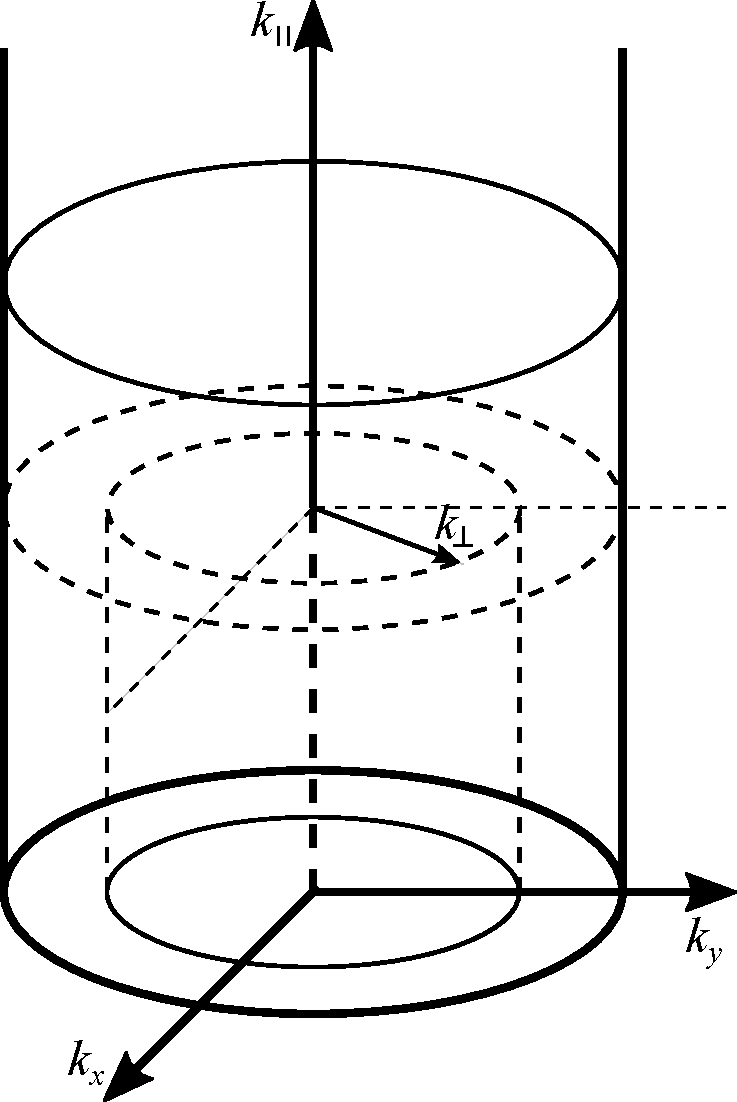
\includegraphics[width=0.35\textwidth]{ps2d-annuli-diagram}
  \bicaption[计算二维功率谱的示意图]{%
    计算二维功率谱 $P(k_{\bot}, k_{\parallel})$ 的示意图:
    在三维功率谱 $P(\B{k}_{\bot}, k_{\parallel})$ 的每一个 $k_{\parallel}$ 平面里,
    按一系列圆环(半径为 $k_{\bot} = |\B{k}_{\bot}|$)将功率平均.
  }{%
    A diagram showing the calculation of the \ac{2d} power spectrum
    $P(k_{\bot}, k_{\parallel})$:
    in each $k_{\parallel}$ plane of the \ac{3d} power spectrum,
    average the powers in a series of annuli with radius of
    $k_{\bot} = |\B{k}_{\bot}|$.
    \\\textcopyright{}
    \citeay{thyagarajan2013}.
  }
  \label{fig:ps2d-calculation}
\end{figure}

EoR 信号的\ac{imgcube} $I_{\R{eor}}(\B{\theta}, \nu)$
的三个维度在本质上是相同的,均映射为中性氢的空间坐标.
但是对于前景的\ac{imgcube} $I_{\R{fg}}(\B{\theta}, \nu)$,
频率维度 $\nu$ 表示前景辐射源的频谱(通常为连续谱),
与两个空间维度 $\B{\theta}$ 完全不同,两者之间也是相互独立的.
因此,一个更好的方法是保持三维功率谱 $P(\B{k}_{\bot}, k_{\parallel})$
的 $k_{\parallel}$ 维度不变,只将两个空间维度 $\B{k}_{\bot}$ 压缩至一维.
具体的做法是:
如\autoref{fig:ps2d-calculation} 所示,
在三维功率谱的每一个 $k_{\parallel}$ 平面里,取一系列圆环将功率平均,
得到二维功率谱 $P(k_{\bot}, k_{\parallel})$,
其中 $k_{\bot} = |\B{k}_{\bot}|$ 是圆环的半径 \cite{datta2010,thyagarajan2013}.

在二维功率谱上,EoR 信号因具有不光滑的频谱而主要分布在 $k_{\parallel}$ 较大的区域,
频谱光滑的前景则主要分布在 $k_{\parallel}$ 较小的区域,
因此可以避开这些受前景严重污染的区域,在相对干净的区域开展 EoR 信号的探测和研究,
这为克服强烈的前景干扰提供了极大的便利.
由于这个独特优势,二维功率谱目前已成为分析 EoR 观测数据的最常用工具
\cite{trott2012,thyagarajan2013,barry2016,beardsley2016,trott2016,patil2017}.


%=====================================================================
\section{探测方法}
\label{sec:det-methods}

目前探测 EoR 信号的方法主要有以下三种,由易到难分别为:
\begin{enumerate}
  \item 测量全天总功率;
  \item 测量功率谱;
  \item 直接获取再电离区域的图像,即 \ac{21cm-tomography}.
\end{enumerate}

第一种方法仅测量 EoR 信号的全天总功率随红移(即观测频率)的变化,
所得结果可以用于推断物质的电离过程,帮助检验和约束再电离模型
\cite{pritchard2012,liu2016}.
该方法相对简单易行,通常采用小型专用设备,一般包含单个或少量天线.
目前已有一批采用该方法的 EoR 探测实验,主要包括
位于澳大利亚的 \ac{edges} \cite{bowman2008} 和
\ac{bighorns} \cite{sokolowski2015}、
位于美国的 \ac{leda} \cite{greenhill2012}、
位于墨西哥的 \ac{sci-hi} \cite{voytek2014}
以及位于印度的 \ac{saras} \cite{singh2018}.
值得一提的是,\acs{edges} 在 2018 年初报导称发现全天平均射电信号在 \SI{78}{\MHz}
附近存在吸收,该吸收信号所处位置大致符合早期恒星所引发的 21\,cm 信号,
但其强度是目前理论预测值的两倍以上 \cite{bowman2018}.

后两种方法则进一步测量 EoR 信号的统计分布规律甚至三维图像,能够提供更加全面丰富
的信息用于系统性地研究\acl{eor}.
尽管这两种测量方法更加强大有效,但需要大型低频干涉阵列,
如 \autoref{sec:instruments} 所介绍的主要干涉阵列,
其中仅有 \acs{ska} 将拥有足够高的灵敏度实现对再电离区域的直接成像观测.


%=====================================================================
\section{主要困难}
\label{sec:det-difficulties}

EoR 探测实验,尤其是采用干涉阵列,面临着一系列困难.
这些困难可主要分为以下几类:
\begin{itemize}
\item
\emph{前景干扰:}
源自银河系以及河外源的前景辐射非常强烈,可达数百 \si{\kelvin},
是 EoR 信号(仅约几 \si{\mK} 至几十 \si{\mK})的 \numrange{4}{5} 个数量级
\cite{morales2010}.
虽然对干涉阵列而言重要的是辐射的空间涨落幅度而非其平均强度,
但是前景辐射的涨落幅度仍达数 \si{\kelvin} 到数十 \si{\kelvin},
远远压制了待测 EoR 信号 \cite{zaroubi2013}.
\autoref{fig:eor-foregrounds} 显示了主要的前景成分及其在
\SI{120}{\MHz} 处的强度.
因此,即便是轻微的前景处理不当,都会导致微弱的 EoR 信号被淹没而无法被捕捉到.
此外,部分前景成分(如银河系\ac{rad-syn})存在一定程度的偏振,
该偏振成分可能发生泄漏而影响前景强度的测量,即\ac{pl}效应 \cite{cotton1999},
导致前景的频谱结构复杂化而变得更加难以处理
\cite{jelic2014,asad2015,asad2016,asad2018,gehlot2018}.
如何处理强烈的前景干扰并成功分离 EoR 信号,
是目前 EoR 探测领域的一个关键任务,
不仅需要系统深入地理解各个前景成分的特征
\cite{jelic2008,jelic2010,wang2010,liu2012,offringa2016,
  carroll2016,murray2017,procopio2017,spinelli2018},
还需要研发有效的前景扣除与信号分离算法
\cite{wang2006,jelic2008,harker2009,liu2009fgrm,chapman2012,chapman2013,
  gu2013,wang2013,bonaldi2015,chapman2015,chapman2016,mertens2018}.

\begin{figure}[tbp]
  \centering
  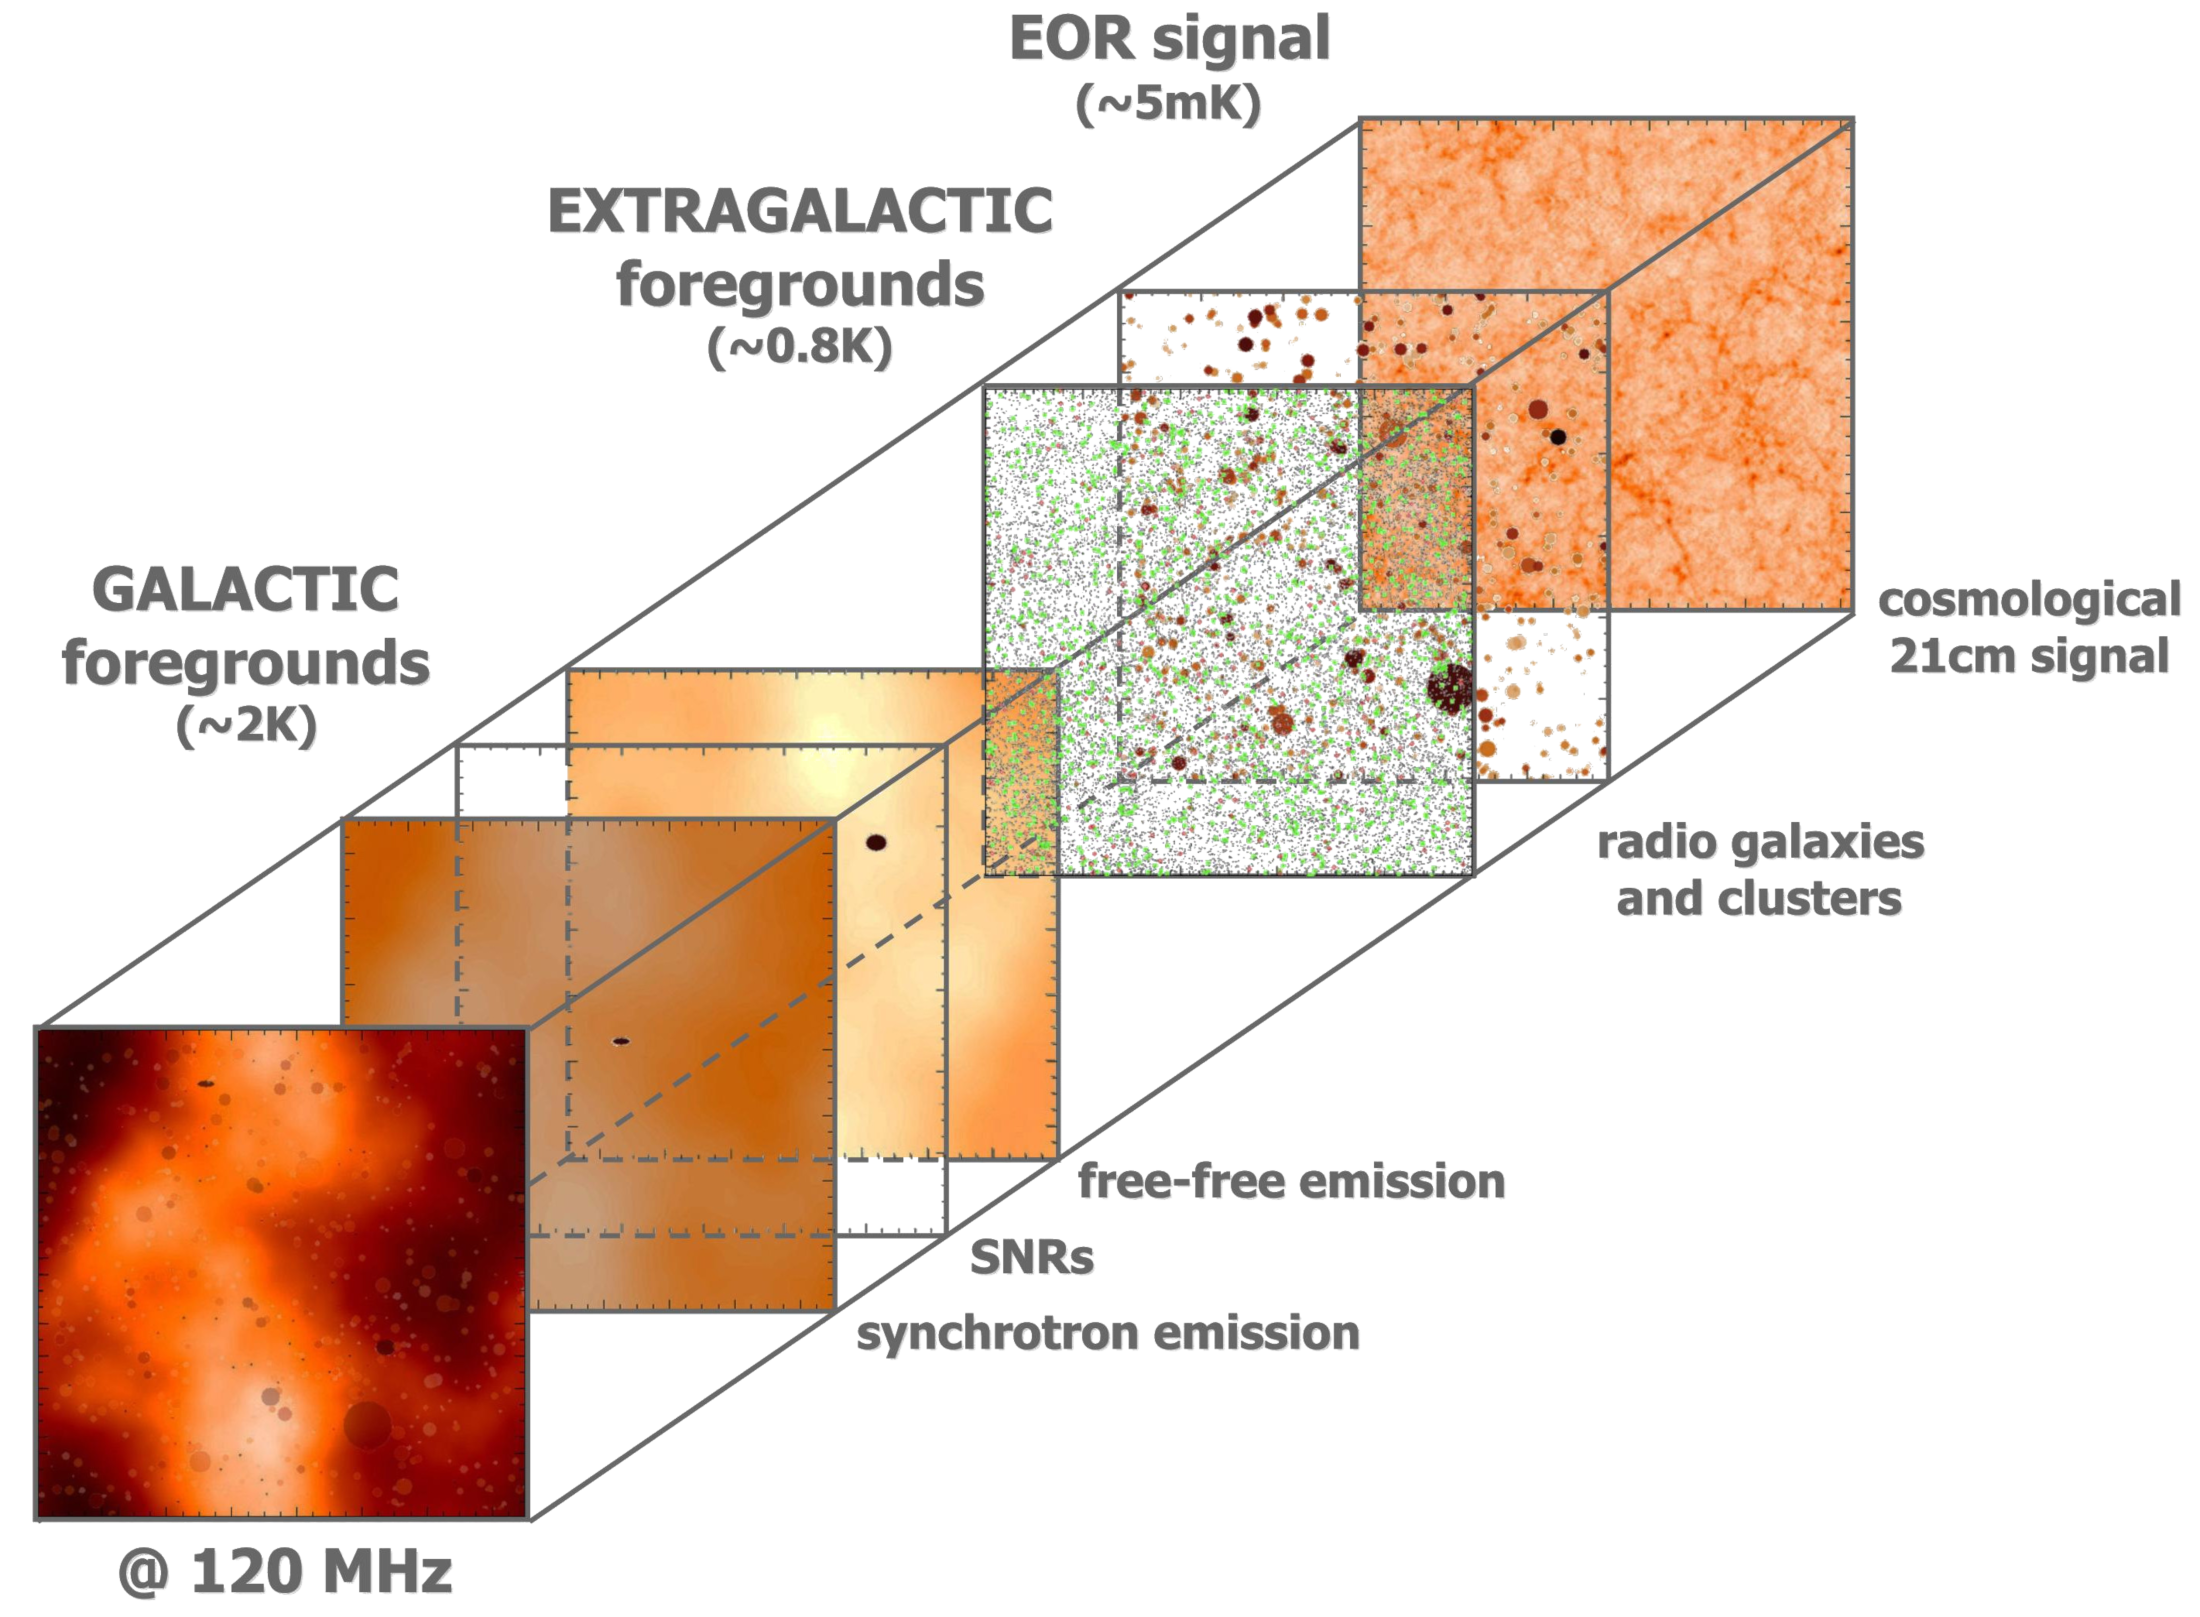
\includegraphics[width=0.7\textwidth]{eor-foregrounds}
  \bicaption[主要前景成分及其强度示意图]{%
    主要前景成分以及强度示意图.
    图中的数值代表在 \SI{120}{\MHz} 处的\acs*{rms}值.
  }{%
    A diagram showing the major foreground components contaminating
    the EoR signal.
    The numbers in the figure represent the root-mean-square values
    at \SI{120}{\MHz}.
    \\\textcopyright{}
    \citeay{zaroubi2013}, \S\,5.5.
  }
  \label{fig:eor-foregrounds}
\end{figure}

%.......................................
\item
\emph{人工源的\acl{rfi}:}
随着科技的进步和社会的发展,人类活动产生的无线电波已在地球上无处不在,
对射电天文观测产生了严重的\acf{rfi}.
这些人工源主要有:\ac{am}和\ac{fm}广播、卫星通信、\ac{gps}信号、
对讲机、手机、移动通信基站、航空通信、雷达、等等.
虽然 EoR 探测设备通常建设在人烟稀少的射电宁静区域,但是仍不可避免受到
人工源的 \ac{rfi},甚至由月亮以及太空碎片反射回来的无线电波都可能
对 EoR 观测产生一定程度的影响 \cite{mcKinley2013,tingay2013rfi}.
如\autoref{fig:rfi-mwa} 所示的是 MWA 在其各子频段的\ac{vis}数据
被标记为 \ac{rfi} 的比例,其中突显了\ac{fm}广播、卫星通信以及数字电视
等干扰源对 EoR 探测所造成的影响.
\ac{rfi} 的强度通常会高出天空信号的若干个数量级,并且实时发生变化 \cite{bentum2011}.
目前常用的一种办法是识别并屏蔽存在明显 \ac{rfi} 的时间和频率片段
\cite{fridman2001,offringa2010,offringa2012,prasad2012,akeret2017},
但是残留的干扰可能会对前景处理以及 EoR 信号测量均产生严重影响 \cite{offringa2015}.

\begin{figure}[tbp]
  \centering
  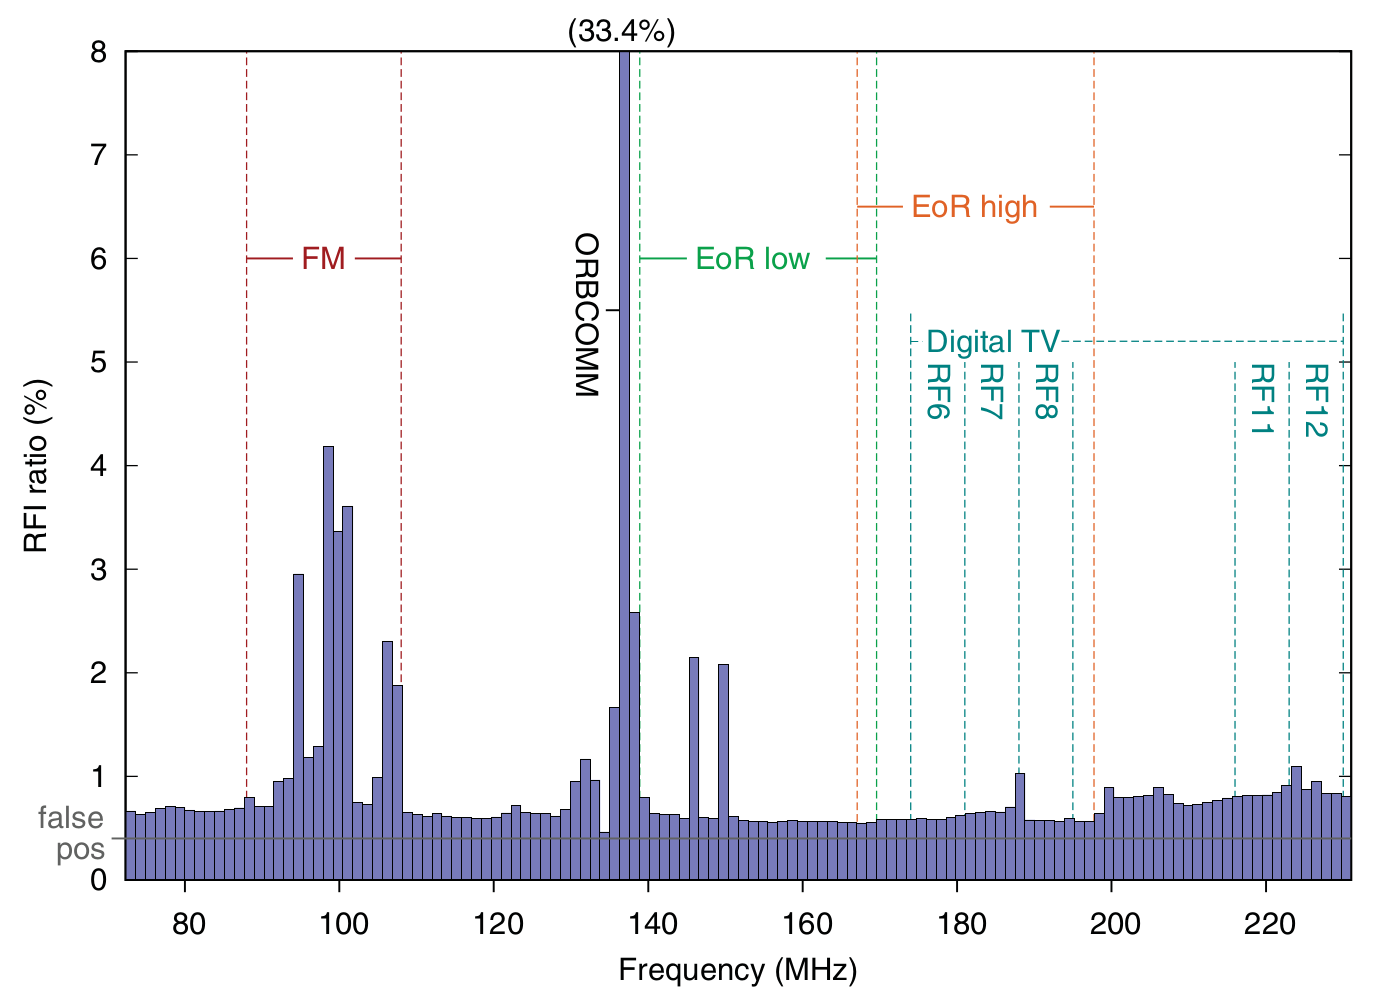
\includegraphics[width=0.7\textwidth]{RFI-MWA}
  \bicaption[MWA 各子频段内的 RFI 比例]{%
    MWA 各子频段的\acs*{vis}数据被标记为 \acs*{rfi} 的比例.
  }{%
    The \acs*{rfi} occupancy, calculated as the percentage of
    visibilities that are detected as \acs*{rfi} by the flagger,
    per sub-band for the MWA.
    \\\textcopyright{}
    \citeay{offringa2015}.
  }
  \label{fig:rfi-mwa}
\end{figure}

%.......................................
\item
\emph{电离层干扰:}
\acf{ionosphere}是地球大气层上部被太阳辐射电离的部分,从约 \SI{60}{\km}
延伸至约 \SI{1000}{\km} 的高空,覆盖了大气层的\ac{thermosphere}以及
部分\ac{mesosphere}和\ac{exosphere},是地球\ac{magnetosphere}的内界
(如\autoref{fig:ionosphere} 所示).
电离层的大气已经非常稀薄,因此被太阳辐射中的紫外线和 X 射线电离的
空气分子所产生的自由电子在复合前可以短暂地自由活动,形成等离子体,能够对电磁波的
传播产生影响.
在 \SI{< 300}{\MHz} 的低频波段,电离层主要对电磁波产生折射、
传播延迟、Faraday 旋转等影响,导致测量数据存在相位和幅度误差
\cite{intema2009,thompson2017}.
由于主要受太阳活动的影响,电离层的状态会随时间和位置而发生剧烈变化,
因此对干涉阵列各天线产生的干扰程度也存在差异且时刻发生变化.
为了获得高质量的图像,必须实时校准观测数据 \cite{intema2009,jordan2017}.
当干涉阵列的基线很长时,对每个\ac{station}或天线所施加的校准还需要有针对性.
这些将成为 \ac{lofar}、\ac{mwa} 等大型低频干涉阵列的一个严重的计算负担
\cite{intema2009,deGasperin2018}.

\begin{figure}[tbp]
  \centering
  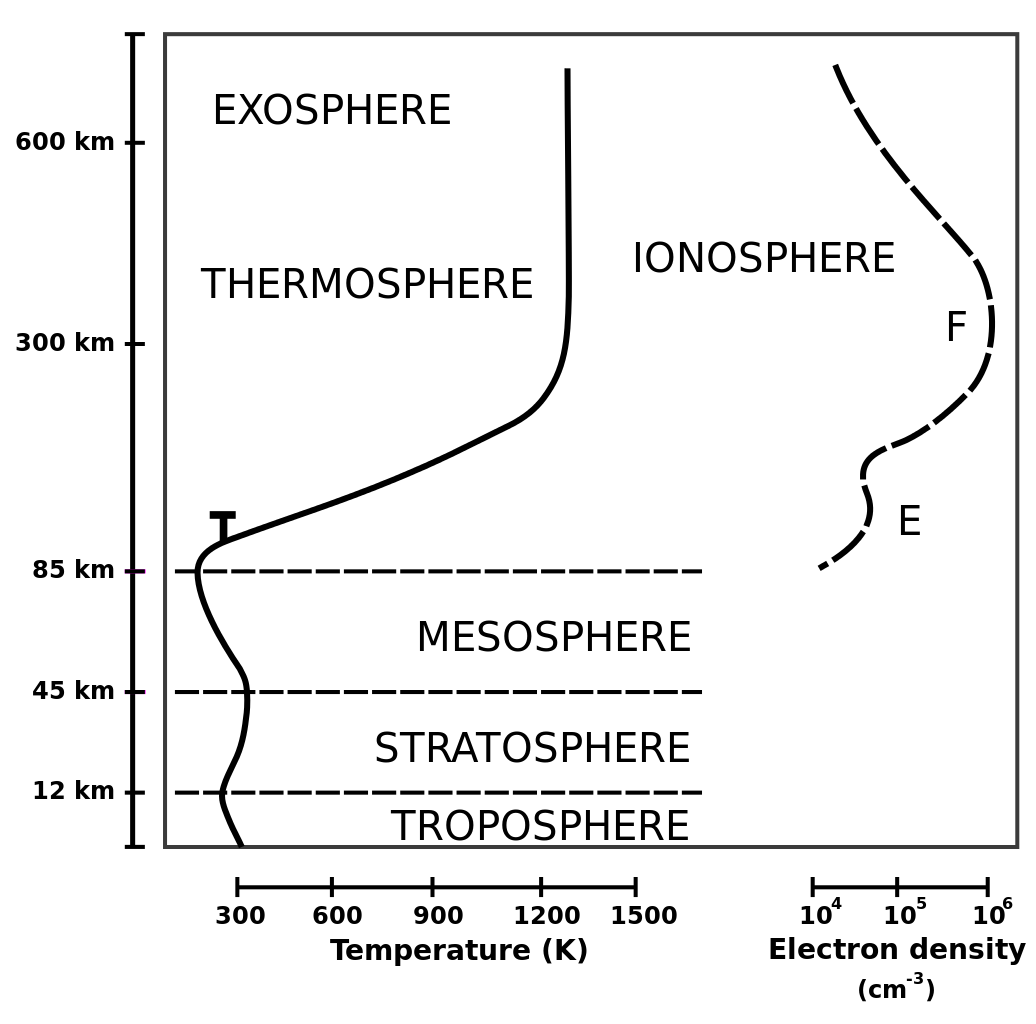
\includegraphics[width=0.5\textwidth]{atmosphere-with-ionosphere}
  \bicaption[大气层和电离层的关系]{%
    地球的大气层和电离层之间的关系.
    电离层是大气层上部被太阳辐射电离的部分.
  }{%
    The relation between Earth's atmosphere and ionosphere, which
    is the ionized part of upper atmosphere.
    \\\textcopyright{}
    Bhamer,
    \url{https://en.wikipedia.org/wiki/File:Atmosphere_with_Ionosphere.svg},
    (2018-10-13), 公有领域.
  }
  \label{fig:ionosphere}
\end{figure}

%.......................................
\item
\emph{仪器效应:}
当代的干涉阵列通常由成千上万根天线组成. 由于生产和安装过程的差异以及随环境和时间的变化,
\ac{station}内每根天线的性能都不可能完全相同,
导致所形成的\ac{beam-station}存在很多不确定因素,
而且各个\ac{station}的波束也互不相同.
对于采用数字\ac{bf}技术的\ac{phased-array}而言,
波束的形态更会随着所指方向而发生大幅变化
\cite{smirnov2011iii,vanWeeren2016,jagannathan2017}.
因此,如果未能全面地校准\ac{beam-station},那么后续对其他仪器效应的校准、
亮点源剥离 (peeling)、前景去除等任务都会受到严重影响 \cite{noordam2004,neben2016}.
此外,还有一系列已知和未知的复杂仪器效应,比如:
显著的旁瓣 \cite{thyagarajan2015,mort2017}、
波束的频率依赖效应 \cite{liu2009ps,datta2010,morales2012}
(另见 \autoref{sec:eor-window} 和 \autoref{sec:fdeffect})、
\ac{pl} \cite{asad2015,asad2016,asad2018,lenc2017}、
天线响应随频率的变化 \cite{bernardi2015,trott2017}、
信号传输过程中在电缆内的反射 \cite{beardsley2016}.
如何准确有效地校准仪器,发挥出仪器的设计性能,是目前最迫切的任务之一
\cite{wijnholds2010} (ref???).

%.......................................
\item
\emph{海量数据:}
大型的干涉阵列将产生海量数据,如 SKA1-Low 的数据流量预计高达 TB/s,
由此引发出一系列难题 \cite{norris2011} (ref???),比如:
如何对原始数据进行实时相关处理?
如何传输和存储如此海量的数据?
如何实现有效的数字\ac{bf}和多波束技术?
如何进行海量数据的校准处理?
如何处理海量数据实现大视场高动态范围成像?
缓解或解决这些问题,不仅依赖于更快更高效的计算资源 \cite{magro2014,vermij2017},
建设新型的数据中心 \cite{chrysostomou2018},
还需要研发新算法以及编写新软件,优化数据处理流程,充分利用大规模并行计算资源
\cite{morales2009,gunst2018} (ref???).

\end{itemize}


%=====================================================================
\section{主要前景成分}
\label{sec:fg-intro}

%---------------------------------------------------------------------
\subsection{银河系同步辐射}

\emph{银河系\acs{rad-syn} (Galactic synchrotron radiation)}
是由弥散于银河系内的高能带电粒子在磁场中发生加速运动而产生的,
是低频射电波段 ($\gtrsim \SI{1}{\GHz}$) 最明亮的前景成分
\cite{bernardi2009,ghosh2012}.
在 \SI{150}{\MHz} 处,即使是高银纬辐射较弱的区域,
银河系同步辐射亦占全部前景辐射的 \SI{\sim 70}{\percent} \cite{shaver1999}.
\autoref{fig:galactic-syn} 上栏显示了由 \citeay{remazeilles2015}
重新处理的 Haslam \SI{408}{\MHz} 巡天图 \cite{haslam1982},
可见银河系同步辐射具有明显的大尺度(约在度以上)子结构,
这将在\ac{ps}的大尺度区域对 EoR 信号产生严重污染.

银河系同步辐射的频谱近似为幂律形式,但谱指数随天空区域而变化,
如\autoref{fig:galactic-syn} 下栏所示.
在高银纬区域,\SIrange{100}{200}{\MHz} 范围内的平均谱指数
$\acs{spec-index}_{\R{syn}} \sim \num{2.5 +- 0.1}$ \cite{rogers2008}.

\begin{figure}[tbp]
  \centering
  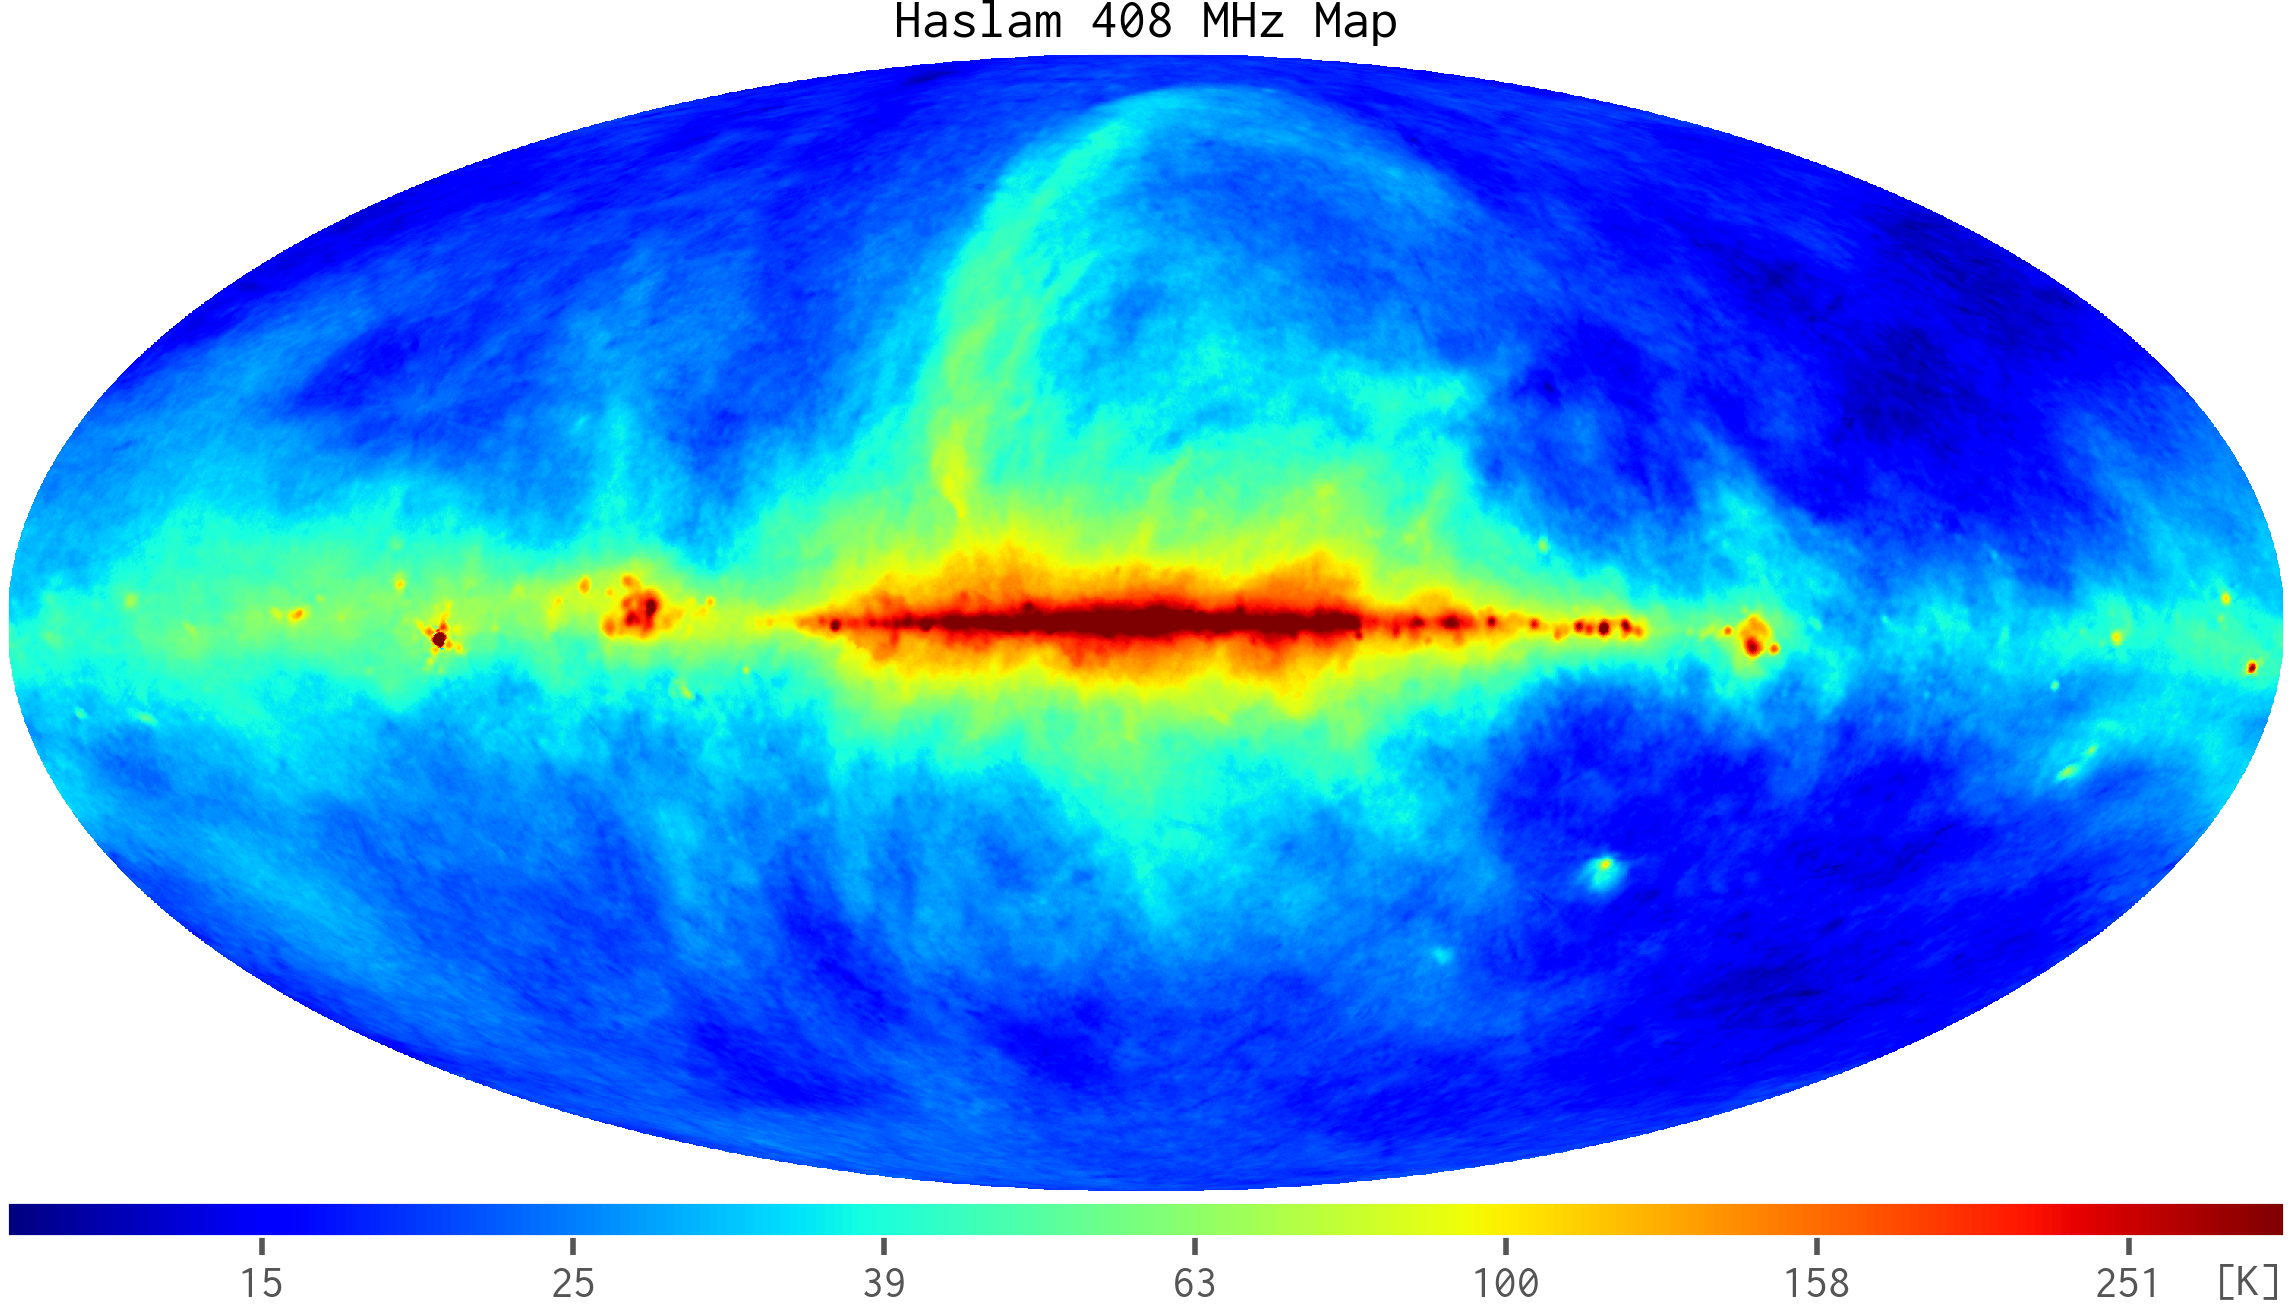
\includegraphics[width=0.9\textwidth]{galactic-haslam408}
  \\\medskip
  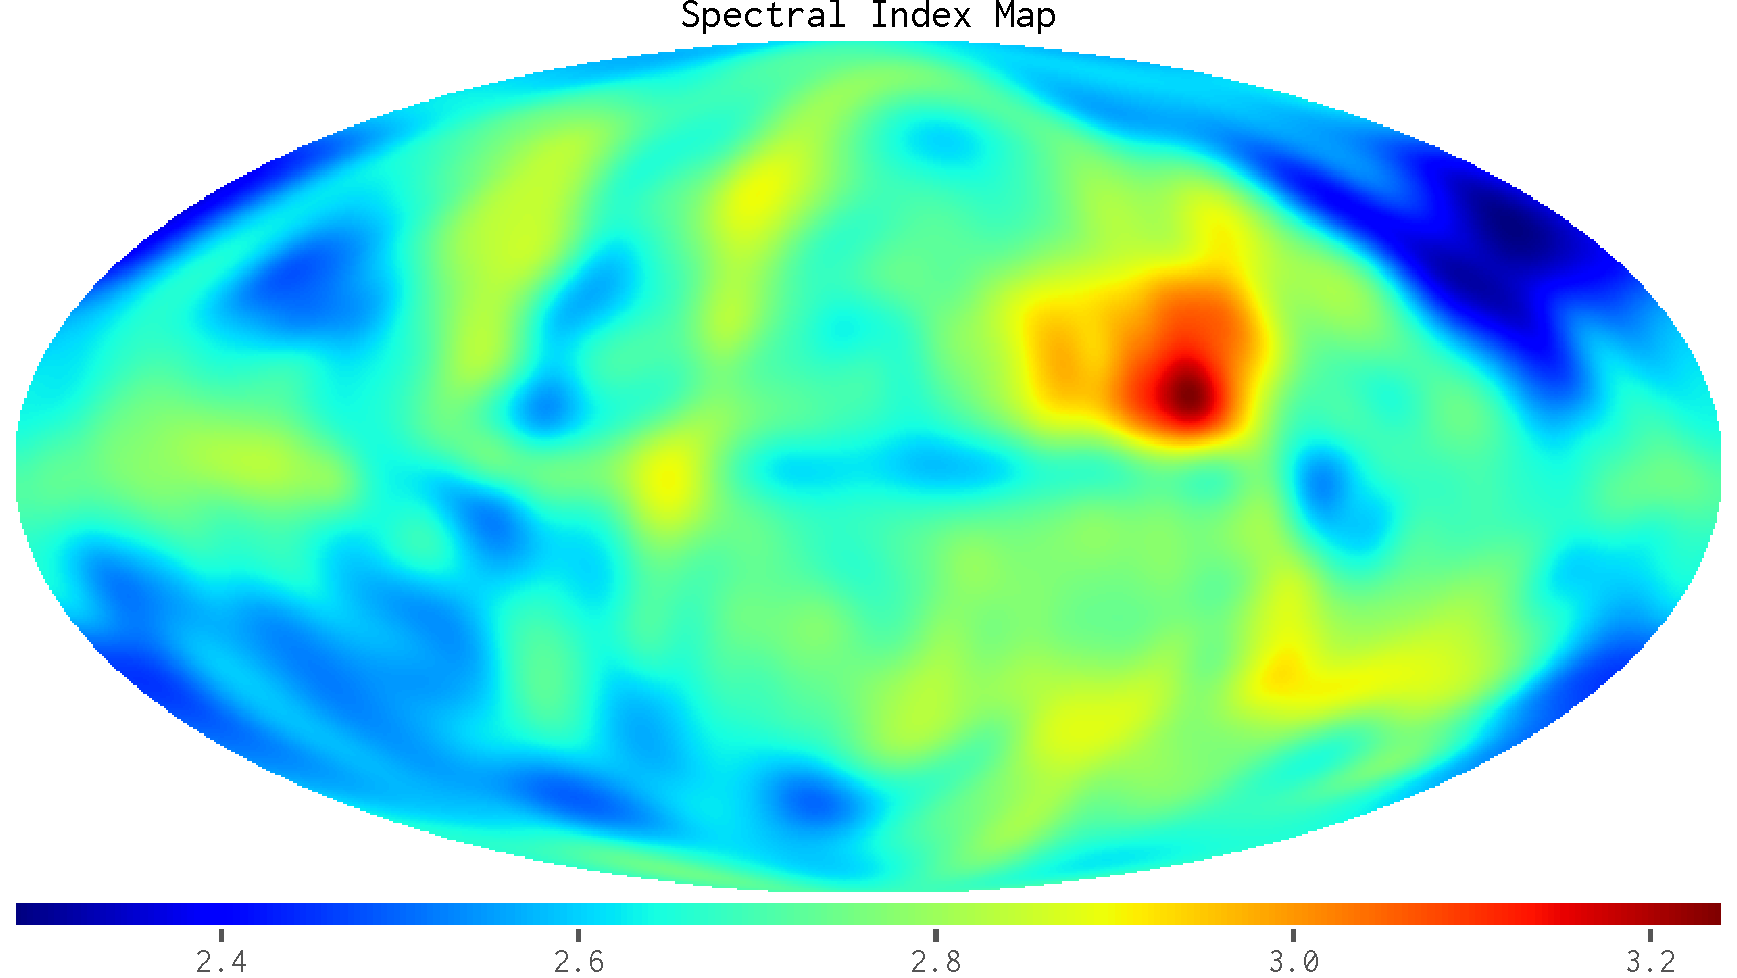
\includegraphics[width=0.9\textwidth]{galactic-spec-index}
  \bicaption[银河系同步辐射的 \SI{408}{\MHz} 巡天图和谱指数图]{%
    \uline{(上栏)}
    由 \citeay{remazeilles2015} 重新处理的 Haslam \SI{408}{\MHz} 巡天图,
    显示了银河系同步辐射的强度分布.
    \uline{(下栏)}
    由 \citeay{giardino2002} 处理得到的银河系同步辐射的谱指数全天分布图,
    利用了 \SI{408}{\MHz} 全天图、\SI{1420}{\MHz} 北天图 \cite{reich1986}
    以及 \SI{2326}{\MHz} 南天图 \cite{jonas1998}.
  }{%
    \emph{(Upper)} The Haslam \SI{408}{\MHz} all-sky map
    reprocessed by \citeay{remazeilles2015} shows the
    Galactic synchrotron radiation.
    \emph{(Lower)} The synchrotron spectral index map obtained
    by \citeay{giardino2002} by utilizing the \SI{408}{\MHz} all-sky map,
    the \SI{1420}{\MHz} northern sky survey \cite{reich1986}, and
    the \SI{2326}{\MHz} southern sky survey \cite{jonas1998}.
  }
  \label{fig:galactic-syn}
\end{figure}

在低频射电波段对银河系同步辐射的观测和研究仍然非常有限,
仅有少数几个天区开展了深入观测和研究
\cite{bernardi2009,ghosh2012,iacobelli2013,choudhuri2017},
基于大规模巡天的研究更是匮乏.
由于磁场强度的涨落、高能带电粒子的密度涨落、\ac{ism}的湍流等因素的影响
\cite{waelkens2009,lazarian2012,iacobelli2013},
银河系同步辐射应具有更复杂的小尺度(角分及亚角分)结构,
但是受限于目前的观测数据(Haslam \SI{408}{\MHz} 全天图的分辨率约为 \SI{0.85}{\degree}),
我们对这些细节的了解程度远远不够 \cite{ali2016}.

另一方面,银河系同步辐射具有一定的偏振 \cite{bernardi2009,jelic2014,gehlot2018}.
偏振的辐射通过磁场时,其偏振面会发生旋转,即 Faraday 旋转效应 \cite{rybicki1979},
而且旋转量依赖于辐射频率,因此天线接收到的某一偏振成分
(如 Stokes $Q$ 或 $U$)的强度变化也依赖于频率,
使得其频谱可能变得不光滑.
同时,仪器因其固有的限制而无法完全隔离各偏振成分的测量,
因此会有少量(约 \SI{1}{\percent} ???)偏振辐射\enquote{漏泄}到总辐射强度里,
可能破坏前景频谱的光滑性,阻碍前景的准确扣除
\cite{jelic2010,nunhokee2017,gehlot2018,spinelli2018}.

%---------------------------------------------------------------------
\subsection{银河系自由--自由辐射}

\emph{银河系\acs{rad-ff} (Galactic free--free radiation)}
源自于银河系的\ac{hii}区、\ac{wim}等区域的热电子的\ac{rad-brem}.
因为电子在辐射前后都是自由的(即没有束缚在离子、原子、分子里),
所以\ac{rad-brem}又被称为\ac{rad-ff}.
银河系\ac{rad-ff}的谱指数 $\acs{spec-index}_{\R{ff}} \sim 2.1$,
比\ac{rad-syn}的频谱偏平一点 \cite{dickinson2003}.

在低频射电波段,除了银盘附近区域,
银河系\ac{rad-ff}被淹没在\ac{rad-syn}之中而无法被直接观测到,
所以我们对该辐射成分的了解非常有限.
目前已掌握的有关银河系\ac{rad-ff}的信息主要源自 Hα 巡天 \cite{finkbeiner2003},
因为产生\ac{rad-ff}的电离区域同时也会产生 Hα 辐射,
而且两种辐射的强度之间存在紧密关联,
因此可以利用 Hα 辐射来有效地追踪\ac{rad-ff} \cite{smoot1998,dickinson2003}.
不过 Hα 辐射容易被尘埃吸收,因此需要首先利用尘埃分布图\cite{schlegel1998}
对 Hα 辐射进行修正,然后再推导\ac{rad-ff} \cite{dickinson2003},
如\autoref{fig:galactic-ff} 显示了利用该方法(详见 \autoref{sec:simu-gff})
得到的银河系\ac{rad-ff}在 \SI{150}{\MHz} 的全天图.
但是在银盘附近,Hα 辐射的尘埃吸收修正将因为尘埃多、分布复杂而变得不可靠,
从而无法给出合理的\ac{rad-ff}.

另一种追踪\ac{rad-ff}的方法是利用\ac{rrl}.
因为\ac{rrl}不受尘埃吸收的影响,所以该方法可以顺利用于银盘附近区域,
给出可靠的\ac{rad-ff} \cite{alves2010,alves2012}.
与前面的方法相结合,可以获得银河系\ac{rad-ff}的完整全天图.

尽管银河系\ac{rad-ff}的强度远弱于同步辐射成分,
比如在 \SI{150}{\MHz} 处贡献了总前景辐射的 \SI{\sim 1}{\percent} \cite{shaver1999},
但仍然是重要的 EoR 前景干扰成分,原因有二 \cite{jelic2008}:
(1) 银河系\ac{rad-ff}的强度和涨落仍然远强于 EoR 信号;
(2) 该前景成分的谱指数和子结构与其他前景成分不同.

\begin{figure}[tbp]
  \centering
  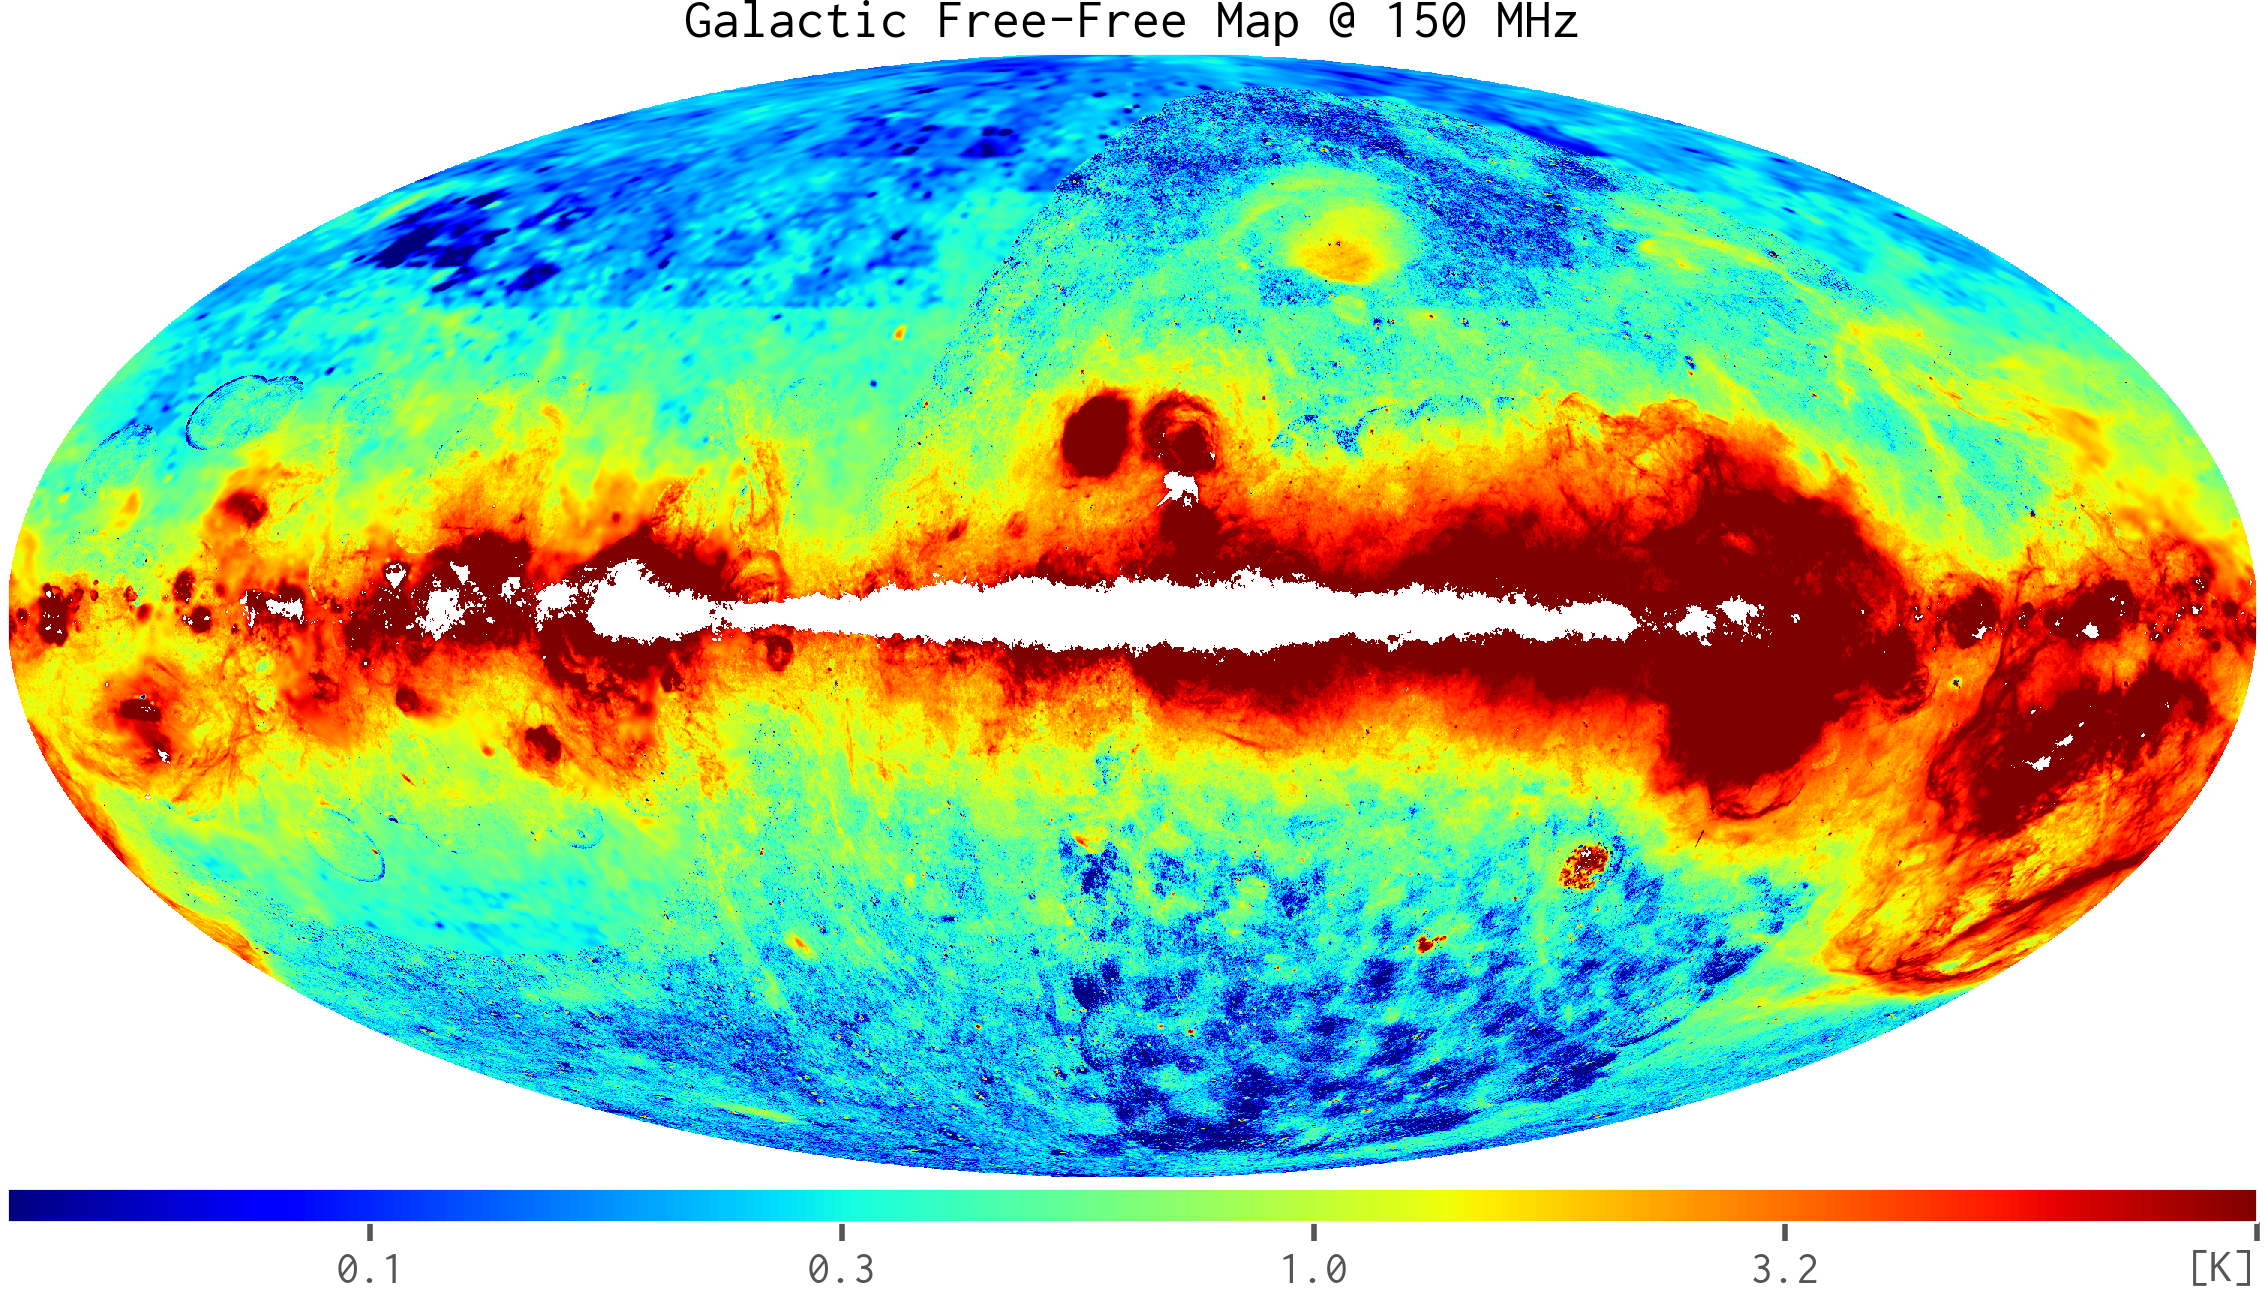
\includegraphics[width=0.9\textwidth]{galactic-freefree}
  \bicaption[银河系自由--自由辐射在 \SI{150}{\MHz} 的全天图]{%
    对 Hα 全天辐射图\cite{finkbeiner2003}修正尘埃吸收后得到的
    银河系自由--自由辐射在 \SI{150}{\MHz} 的强度分布图 \cite{dickinson2003}.
    图中靠近银盘的白色区域由于尘埃吸收修正不可靠而被屏蔽.
  }{%
    The Galactic free--free radiation map at \SI{150}{\MHz}
    derived from the Hα all-sky map \cite{finkbeiner2003}
    with dust absorption corrected \cite{dickinson2003}.
    The white regions near the Galactic plane are masked due to
    the large uncertainty about the correction for dust absorption.
  }
  \label{fig:galactic-ff}
\end{figure}

%---------------------------------------------------------------------
\subsection{河外点源}

除银河系的弥散辐射(\ac{rad-syn}和\ac{rad-ff})之外,最强的前景干扰源
便是数目极多的\emph{河外\acs{src-point} (extragalactic point source)},
这些\ac{src-point}产生的辐射在 \SI{150}{\MHz} 处贡献了总前景辐射的
\SI{\sim 27}{\percent} \cite{shaver1999}.
在\ac{ps}的小尺度(亚角分)区域,河外点源更是成为最强、最难处理的前景成分 (ref???).
如\autoref{fig:mwa-eor0} 显示了 MWA EoR0 天区的深度曝光图像 \cite{offringa2016},
可见密布的点源.

\begin{figure}[tbp]
  \centering
  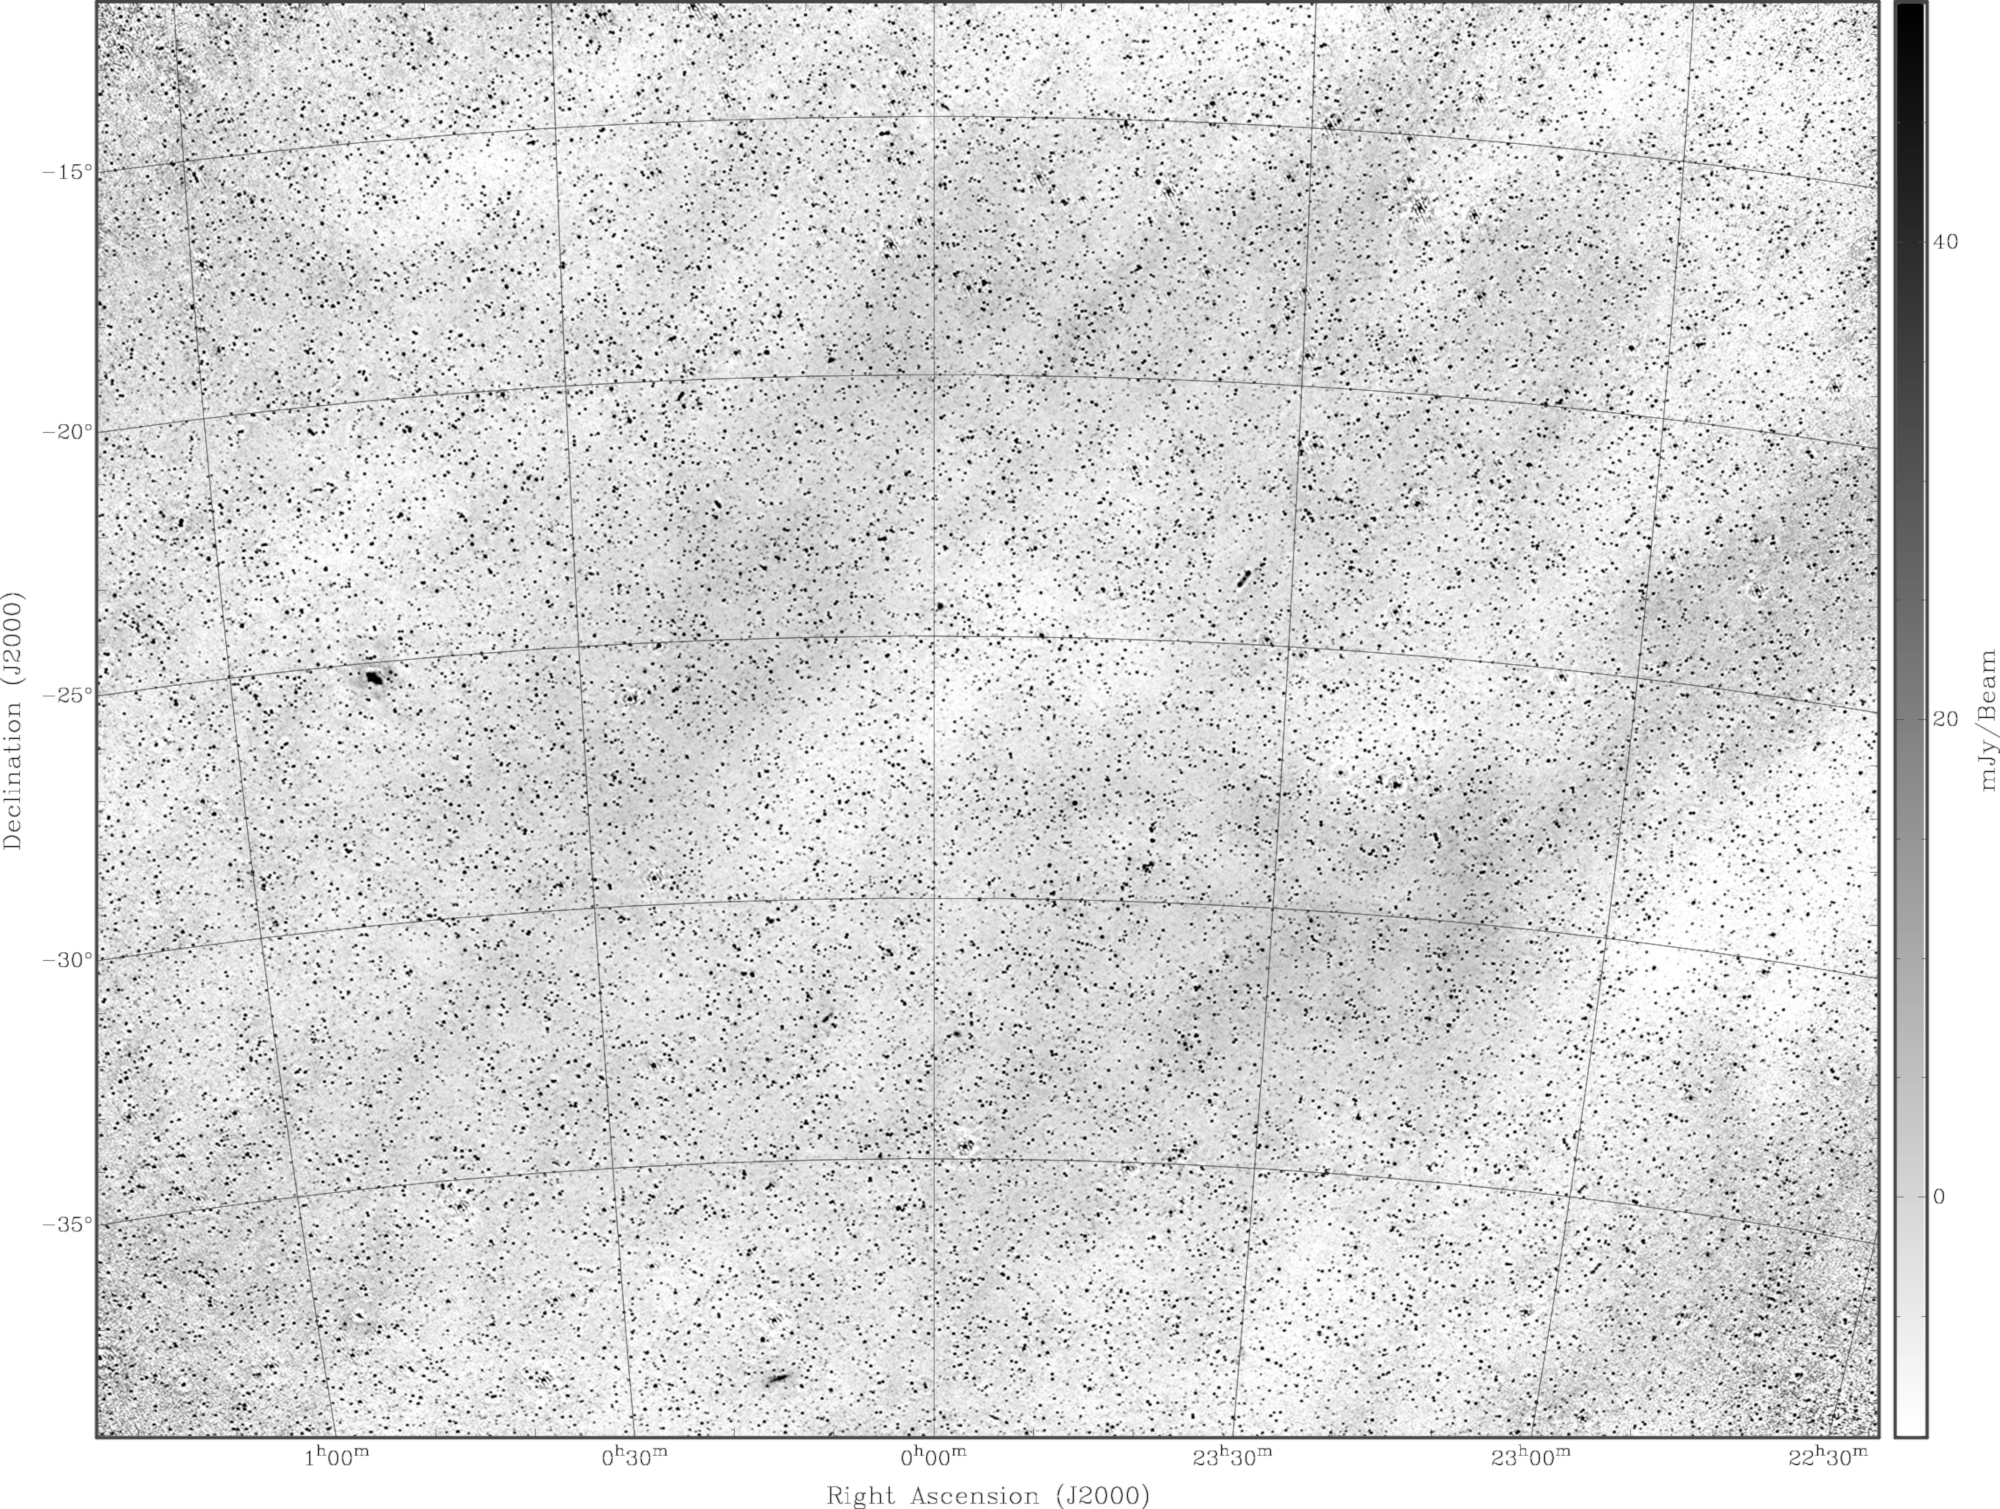
\includegraphics[width=\textwidth]{MWA-EoR0-fullbw}
  \bicaption[MWA EoR0 天区的深度曝光图像]{%
    MWA 对 EoR0 天区 (R.A. = \SI{0}{\degree}, Dec.\@ = \SI{-27}{\degree})
    累计观测 \SI{45}{\hour} 获得的波束修正后的图像,大小约为 \SI{45 x 30}{\degree}.
  }{%
    The beam-corrected map of the EoR0 field
    (R.A. = \SI{0}{\degree}, Dec.\@ = \SI{-27}{\degree}) obtained by
    the MWA after \SI{45}{\hour} of integration time.
    The image size is about \SI{45 x 30}{\degree}.
    \\\textcopyright{}
    \citeay{offringa2016}.
  }
  \label{fig:mwa-eor0}
\end{figure}

% XXX/FIXME!
河外点源可大致分为以下几类 \cite{snellen2000,wilman2008,wang2010}:
(1) 恒星形成星系 (star-forming galaxy),
包括普通晚型星系 (normal late-type galaxy) 和星暴星系 (starburst galaxy);
(2) 射电宁静 (radio-quiet) \ac{agn};
(3) \ac{fr} I 型和 II 型 \ac{agn};
(4) GHz 倒转谱 (GHz-peaked-spectrum) \ac{agn};
(5) 致密陡谱 (compact steep-spectrum) \ac{agn}.
其中 \ac{fr} I 型和 II 型 \ac{agn} 具有强烈的\ac{jet}或射电瓣 (lobe),
呈现复杂的形态结构,所以\enquote{点源}这一命名并不准确,
主要是为了与下文(\autoref{sec:eg-extended})将要介绍的\enquote{展源}区分开来.

目前的低频观测结果显示点源的频谱是光滑的,没有明显的谱线结构 \cite{offringa2016}.
但是不同类别的点源具有不同的谱指数和频谱形态.
还有小部分点源的辐射具有显著偏振,所以观测得到的频谱的光滑性会受到\ac{pl}的影响
\cite{geil2011,vanEck2018}.
此外,河外点源的成团效应 (clustering effect) 会改变其功率谱,
该效应需要被仔细考虑以获得准确的 EoR 信号功率谱
\cite{diMatteo2004,liu2011,murray2017}.

%---------------------------------------------------------------------
\subsection{河外展源}
\label{sec:eg-extended}

\ac{gc}由成百上千个成员星系、弥漫于成员星系之间的 \ac{icm} 以及暗物质组成
\cite{sarazin1986,bohringer2010}.
自 1959 年首次在 Coma 星系团中发现了尺度约 \si{Mpc} 的弥散射电辐射 \cite{large1959},
目前已在百来个星系团中探测到了弥散射电辐射 \cite{feretti2012,vanWeeren2019},
根据其尺度、形态、位置等特征,可大致分为以下三类
\cite{feretti2012,kale2016}:
\begin{itemize}
  \item \emph{\acf{rh}}:
    位于星系团的中央区域,尺度达 \si{\Mpc} 量级,形态比较规则,目前只发现于并合星系团中.
    如\autoref{fig:diffuse-emission} 左栏所示.
  \item \emph{\acf{rmh}}:
    位于弛豫冷核星系团的中央区域,通常围绕中央射电星系,尺度为数百 \si{\kpc},形态规则.
    如\autoref{fig:diffuse-emission} 中栏所示.
  \item \emph{\acf{rr}}:
    位于外围区域,尺度亦达 \si{\Mpc} 量级,呈长条不规则形态,辐射具有较强的偏振;
    在并合星系团和弛豫星系团均有发现,在若干星系团中成对出现.
    \autoref{fig:diffuse-emission} 右栏展示了一个双\ac{rr}的情形.
\end{itemize}
此外,在一些星系团中同时观测到了\ac{rh}和\ac{rr}.

\begin{figure}[tbp]
  \centering
  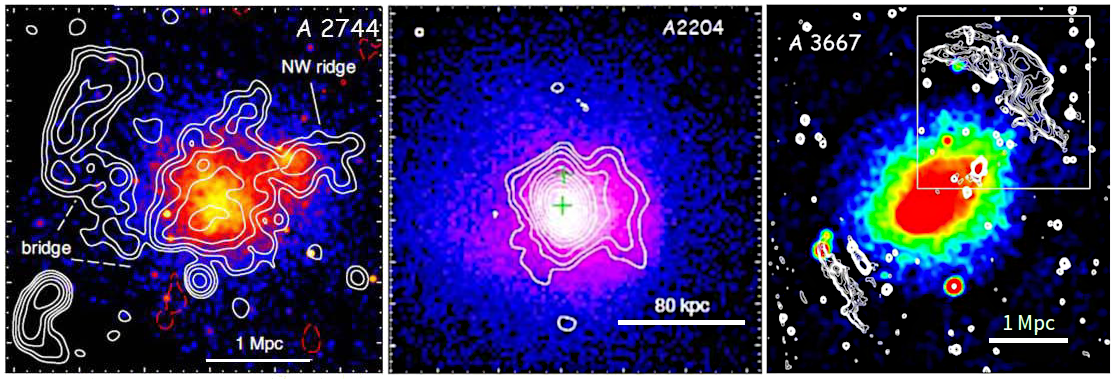
\includegraphics[width=\textwidth]{cluster-diffuse-emission}
  \bicaption[星系团的弥散射电辐射的典型样例]{%
    星系团的弥散射电辐射的典型样例:
    \uline{(左栏)} Abell 2744 中的\acs*{rh};
    \uline{(中栏)} Abell 2204 中的\acs*{rmh};
    \uline{(右栏)} Abell 3667 中的双\acs*{rr}.
    射电辐射以白色等高线标记,并叠加在 X 射线图像上.
  }{%
    Typical examples of diffuse radio emission in galaxy clusters:
    \emph{(left)} a radio halo in Abell 2744;
    \emph{(middle)} a radio mini-halo in Abell 2204;
    \emph{(right)} double radio relics in Abell 3667.
    The radio emissions are marked with white contours and
    superimposed on X-ray images.
    \\\textcopyright{}
    \citeay{brunetti2014}.
  }
  \label{fig:diffuse-emission}
\end{figure}

在星系团中发现弥散射电辐射表明
\ac{icm} 除了包含由高温 ($\gtrsim \SI{1}{\keV}$) 等离子气体构成的热成分,
还存在一个由高能电子 (Lorentz 因子 $\acs{g} > \num{e3}$) 构成的非热成分
(non-thermal component).
这些高能电子弥散于整个星系团,在约 \si{\uG} 的微弱磁场中产生同步辐射,
形成上述大尺度\ac{src-extended}.
电子的能量越高,由于同步辐射以及对 \ac{cmb} 光子的逆 Compton 散射而损失能量的速率越快,
寿命也就越短.
因此,相比高频波段 ($\gtrsim\si{\GHz}$),
\ac{icm} 展源在数百 MHz 的低频波段更容易形成且具有更长的寿命.
以\ac{rh}为例,SKA1-Low 预计将发现约 2500 个 \cite{cassano2015},
远远超过目前已发现的总数 (65 个已确认,另有 28 个候选 \cite{vanWeeren2019}).
尽管 \ac{icm} 展源相比银河系辐射和亮点源来说比较微弱,
但考虑到该前景成分的尺度较大(若干角分)、形态结构复杂、数目较多等特点,
将在\ac{ps}的角分尺度上对 EoR 信号的测量产生严重干扰,
是一个待仔细研究的重要前景成分 \cite{diMatteo2004,gleser2008}.

除了\ac{gc},潜在的河外\ac{src-extended}还包括\ac{sc}和\ac{lsf}.
在这些宇宙大尺度结构里分布着温度约为 \SIrange{e5}{e7}{\kelvin} 的\ac{whim}
和强度约为 \SIrange{10}{100}{\nano\gauss} 的极微弱磁场 \cite{vazza2015}.
在物质落入这些宇宙大尺度结构的过程中、或者物质沿着大尺度结构流动形成星系团等结构时,
会产生较强的激波 (Mach 数约为 ???),从而加速粒子并产生同步辐射 (ref???).
目前还没有获得这些大尺度结构的射电观测证据,SKA 将有能力打破这个局面,
打开研究分布在\ac{sc}和\ac{lsf}的 \ac{igm} 的大门 \cite{vazza2015}.
另一方面,源自这些大尺度结构的射电辐射将如何影响 EoR 信号的探测,
亦是一个值得探讨的问题.


%=====================================================================
\section{前景处理方法}
\label{sec:fg-methods}

微弱的 EoR 信号被强烈的前景污染所淹没是 EoR 探测实验所面临的最主要困难之一.
如何有效地解决此前景污染难题,是成功探测 EoR 信号的关键.
尽管前景污染的强度高达 EoR 信号的 \numrange{4}{5} 个数量级,
但是幸运的是,各前景成分的频谱是相对光滑的,而 EoR 信号的频谱则随频率剧烈震荡,
因为 EoR 信号的频谱反映的是该视线方向上中性氢的分布情况 \cite{diMatteo2002,gnedin2004}.
利用这一关键区别,原则上可以将 EoR 信号从强烈的前景污染中分离出来.

近十余年来,已有一批方法被提出来用于尝试从前景污染中分离出微弱的 EoR 信号.
根据处理前景的策略,可将这些方法大致分为两类 \cite{chapman2015,chapman2016}:
\begin{itemize}
\item \emph{前景扣除法}:
在图像空间或 $uv$ 空间(即 Fourier 空间),
利用前景辐射和 EoR 信号两者明显不同的频谱特征,
对每个像素点沿频率维度(即沿视线方向)识别光滑的前景成分并扣除,从而分离出 EoR 信号.
根据对前景频谱的建模方式,该类方法可进一步分为两小类:
\begin{itemize}
  \item 参数化 (parametric) 方法:
    认为前景频谱可以由一个参数化模型(如低阶多项式)来描述,
    然后用此模型拟合前景频谱并扣除.
    这类方法主要包括多项式拟合法及其变种
    \cite{wang2006,jelic2008,liu2009fgrm,wang2013,bonaldi2015}.
  \item 非参数化 (non-parametric) 方法:
    不作前景频谱应符合某一特定参数化模型的假定,
    仅利用前景的频谱特征与 EoR 信号不同来实现两者的分离.
    其中典型的方法有
    Wp 平滑法 \cite{harker2009}、
    \ac{ica} \cite{chapman2012}、
    \ac{gmca} \cite{chapman2013}、
    \ac{cwt} \cite{gu2013}.
\end{itemize}

%.......................................
\item \emph{前景回避法}:
在二维功率谱 $P(\kperp, \klos)$ 上,
频谱光滑的前景将主要分布在 \klos{} 较小的区域.
尽管复杂的仪器效应会将前景在 \kperp{} 模式里的功率\enquote{混合}到 \klos{} 模式里,
导致前景污染将占据二维功率谱的右下方一个楔形区域,
但左上方的区域(即 EoR 窗口)仍然几乎未受前景污染的影响,
详见下文 \autoref{sec:eor-window}.
因此,\ac{fgavd}通过识别并避开受到前景污染的区域,从而实现提取 EoR 信号的目标.
近年来,该方法已得到了较多的关注和研究 \cite{thyagarajan2013,liu2014,liu2014ii,
  barry2016,beardsley2016,trott2016,patil2017}.

\end{itemize}

上述两类方法均有各自的优缺点.
\ac{fgrm}的优点是能够保留 EoR 信号的全部信息,
但缺点是可能无法准确扣除前景污染或者将部分 EoR 信号错误扣除,导致结果出现一定的偏差.
\ac{fgavd}的优点是可以有效避免前景污染对 EoR 探测结果产生的可能偏差,
而主要缺点便是损失了 EoR 信号在 EoR 窗口之外的信息,
牺牲了仪器的灵敏度和利用效率 \cite{pober2014}.
可进一步参见 \citeay{chapman2016} 及其所引文献.

当然,这两类前景处理方法并不冲突,在实际中可以结合使用,
比如先在图像空间或 $uv$ 空间扣除明显的前景污染,
再利用\ac{fgavd}在二维功率谱上提取 EoR 信号 \cite{datta2010}.


%=====================================================================
\section{再电离窗口}
\label{sec:eor-window}

EoR window, foreground wedge, explanation ...

Considering that the signal is isotropic among the sky plane, we can
squeeze these two dimensions into $\kperp \equiv \sqrt{k_x^2 + k_y^2}$ by
cylindrically averaging the 3D power spectrum, and obtained the 2D
cylindrical power spectrum $P(\kperp, \klos)$ with $\klos \equiv k_z$.
The 2D cylindrical power spectrum has the advantage to better separate
the EoR signal from the foreground contamination, which is supposed to
be reside in the lower-right wedge-shape region, therefore defining the
EoR window.


%=====================================================================
\section{小结}

TODO


%% EOF
